\chapter{作品设计与实现}\label{ux7b2cux4e09ux7ae0-ux4f5cux54c1ux8bbeux8ba1ux4e0eux5b9eux73b0}

本章围绕 V-Guard
系统的实际设计与实现展开说明。首先给出系统设计目标和总体架构，然后介绍系统工作流程、功能模块和核心算法流程，最后说明前端页面、后端服务、任务管理、结果展示和历史记录等应用实现。与第二章的技术背景不同，本章重点说明本作品如何被构建成一个可使用、可展示、可评估的完整系统。

\section{系统设计目标}\label{ux7cfbux7edfux8bbeux8ba1ux76eeux6807}

V-Guard
面向公开语音发布前的声音资产保护需求，目标是将主动防护方法封装为普通用户可以直接操作的系统工具。系统不是单独运行的算法脚本，而是围绕用户上传、音频处理、防护生成、效果评估、结果展示和文件导出构建完整应用流程。用户不需要直接理解语音分词器、代理模型组、损失函数或梯度更新等底层细节，即可通过网页页面完成音频保护任务。

系统的第一个目标是支持音频和视频文件上传。在真实应用场景中，用户待保护的数据来源复杂，既可能是个人录音、播客片段、短视频音轨，也可能是企业播报音频或会议录音。因此，系统需要支持常见音频格式和含语音内容的视频文件，并在后端完成格式检测、文件校验和音轨抽取。

系统的第二个目标是支持自动预处理。不同来源文件在采样率、声道数、文件格式、音量大小和音频时长方面可能存在明显差异。如果直接将这些文件输入保护算法，容易造成模型推理不稳定或评估结果不可比。因此，系统需要在进入主动防护流程前完成格式转换、采样率统一、声道统一、音量规范化和长音频切分，将用户上传内容转换为后续模块可统一处理的标准波形数据。

系统的第三个目标是生成受保护音频。受保护音频应在正常听感上尽量保持自然、可懂和可发布，同时在机器模型的语义表示链路和声音身份特征链路中产生一定偏移。系统通过保护扰动生成模块在原始音频上叠加细粒度扰动，使公开发布后的音频降低被未授权语音克隆系统稳定提取的风险。

系统的第四个目标是提供保护效果量化评估。主动防护系统不能只输出一个处理后的音频文件，还应向用户说明保护前后发生了哪些变化。因此，系统从语义识别、声音身份相似度、音频质量和系统性能等角度进行评估，并输出结构化指标。语义识别评估主要包括自动语音识别（ASR，Automatic
Speech Recognition）转写文本对比、词错误率（WER，Word Error
Rate）和字符错误率（CER，Character Error
Rate）；声音身份评估主要包括说话人相似度（Speaker
Similarity）；音频质量评估主要包括信噪比（SNR，Signal-to-Noise
Ratio）、感知语音质量评估（PESQ，Perceptual Evaluation of Speech
Quality）、波形图和频谱图等。

系统的第五个目标是支持前端可视化展示。用户需要通过直观方式理解保护前后音频的差异，而不能只看到抽象指标。因此，系统在结果页面中展示原始音频和受保护音频的试听对比、自动转写文本对比、声音身份相似度变化、音频质量指标、波形变化和频谱变化，使用户能够从听感、语义识别和声音身份三个角度观察保护效果。

系统的第六个目标是支持历史任务查看和结果导出。对于用户而言，语音保护任务往往不是一次性操作，可能需要多次处理、对比不同保护模式或复查历史结果。因此，系统需要为每次处理任务生成任务编号，记录任务状态、原始文件、受保护文件、评估结果和错误日志，并提供历史任务查询、结果复查、保护音频下载和评估结果导出功能。

综上，V-Guard
的系统设计目标可以概括为：以网页端交互为入口，以主动保护生成算法为核心，以多维度评估为支撑，以历史任务和结果导出为闭环，构建一个面向真实语音发布场景的声音资产主动防护系统。

\section{系统总体设计}\label{ux7cfbux7edfux603bux4f53ux8bbeux8ba1}

\subsection{系统架构设计}\label{ux7cfbux7edfux67b6ux6784ux8bbeux8ba1}

V-Guard
采用前后端分离的系统架构。前端负责用户交互、任务提交、状态展示、结果可视化和文件下载；后端负责文件接收、音频预处理、保护扰动生成、评估指标计算、结果存储和接口响应。通过这种结构，系统既能够支撑算法验证，也能够面向作品展示和实际使用提供完整交互流程。

从功能层次看，系统可划分为四层：数据接入层、主动保护层、效果评估层和应用展示层。四层之间按照``输入接入---保护生成---效果评估---结果展示''的顺序组织，共同构成从原始语音上传到受保护音频导出的完整闭环。


\begin{figure}[htbp]
  \centering
  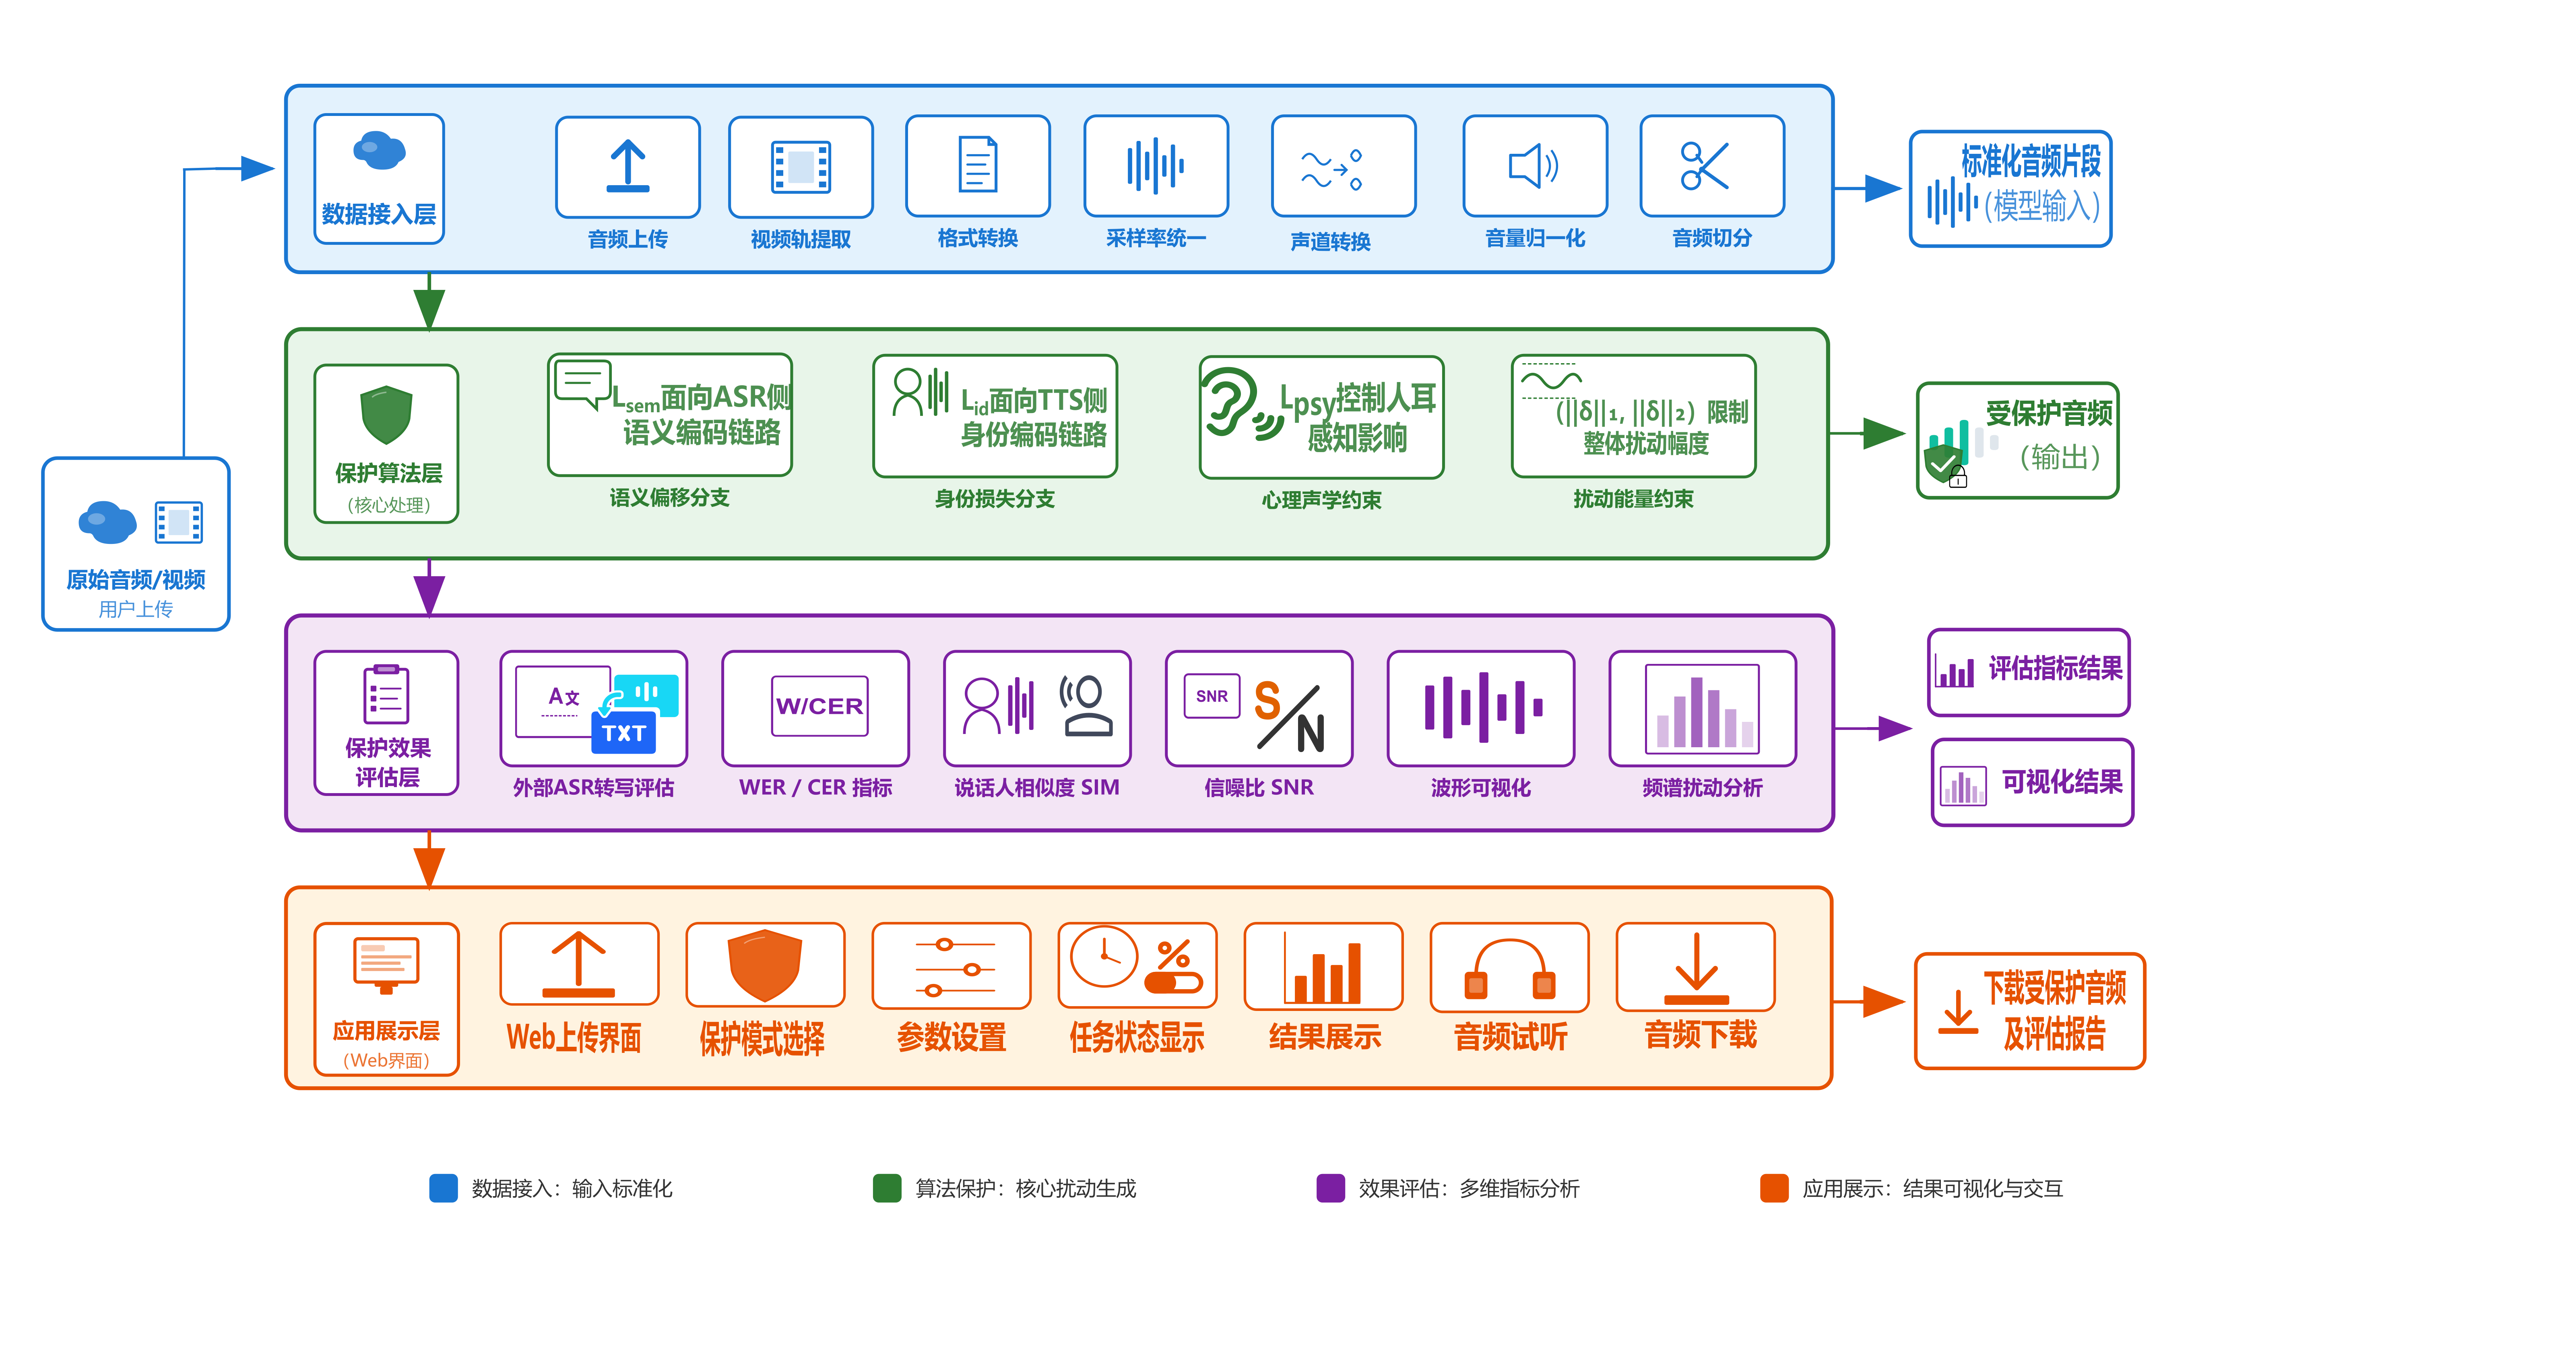
\includegraphics[width=\textwidth,height=0.72\textheight,keepaspectratio]{figures/image15.png}
  \caption{系统总体架构图}
  \label{fig:3-1}
\end{figure}

数据接入层是系统处理流程的入口。该层负责接收用户上传的音频或视频文件，并完成格式检测、合法性校验、音轨抽取、格式转换、采样率统一、声道转换、音量规范化和长音频切分等操作。经过数据接入层处理后，不同来源、不同格式、不同采样率的文件被转换为统一的标准波形数据，为后续主动保护生成和效果评估提供稳定输入。

主动保护层是系统的核心计算层。该层根据用户选择的保护模式和系统参数，在原始音频上生成保护扰动，并输出受保护音频。主动保护层不是简单叠加随机噪声，而是围绕语义表示链路、声音身份特征链路和听感约束共同构建优化目标，使保护音频在机器表示空间中偏离原始音频，同时尽量保持人耳正常听感。

效果评估层负责对保护前后的音频进行多维度分析。该层不直接参与扰动生成，而是为用户判断保护结果提供依据。系统在该层计算
ASR 转写差异、WER /
CER、说话人相似度、SNR、PESQ、波形差异、频谱差异和处理耗时等指标，并将评估结果整理为结构化数据返回前端。

应用展示层面向最终用户提供 Web
化交互界面。用户可以通过浏览器完成文件上传、保护模式选择、任务提交、任务状态查看、结果试听、指标查看、历史任务管理和受保护音频下载。该层将底层算法和评估结果转化为可理解、可操作、可展示的用户流程，是作品落地和答辩演示的主要入口。

\subsection{系统工作流程}\label{ux7cfbux7edfux5de5ux4f5cux6d41ux7a0b}

从用户视角看，V-Guard
的完整工作流程包括上传文件、预处理、选择保护模式、提交保护任务、生成受保护音频、计算评估指标、展示结果和下载文件八个步骤。


\begin{figure}[htbp]
  \centering
  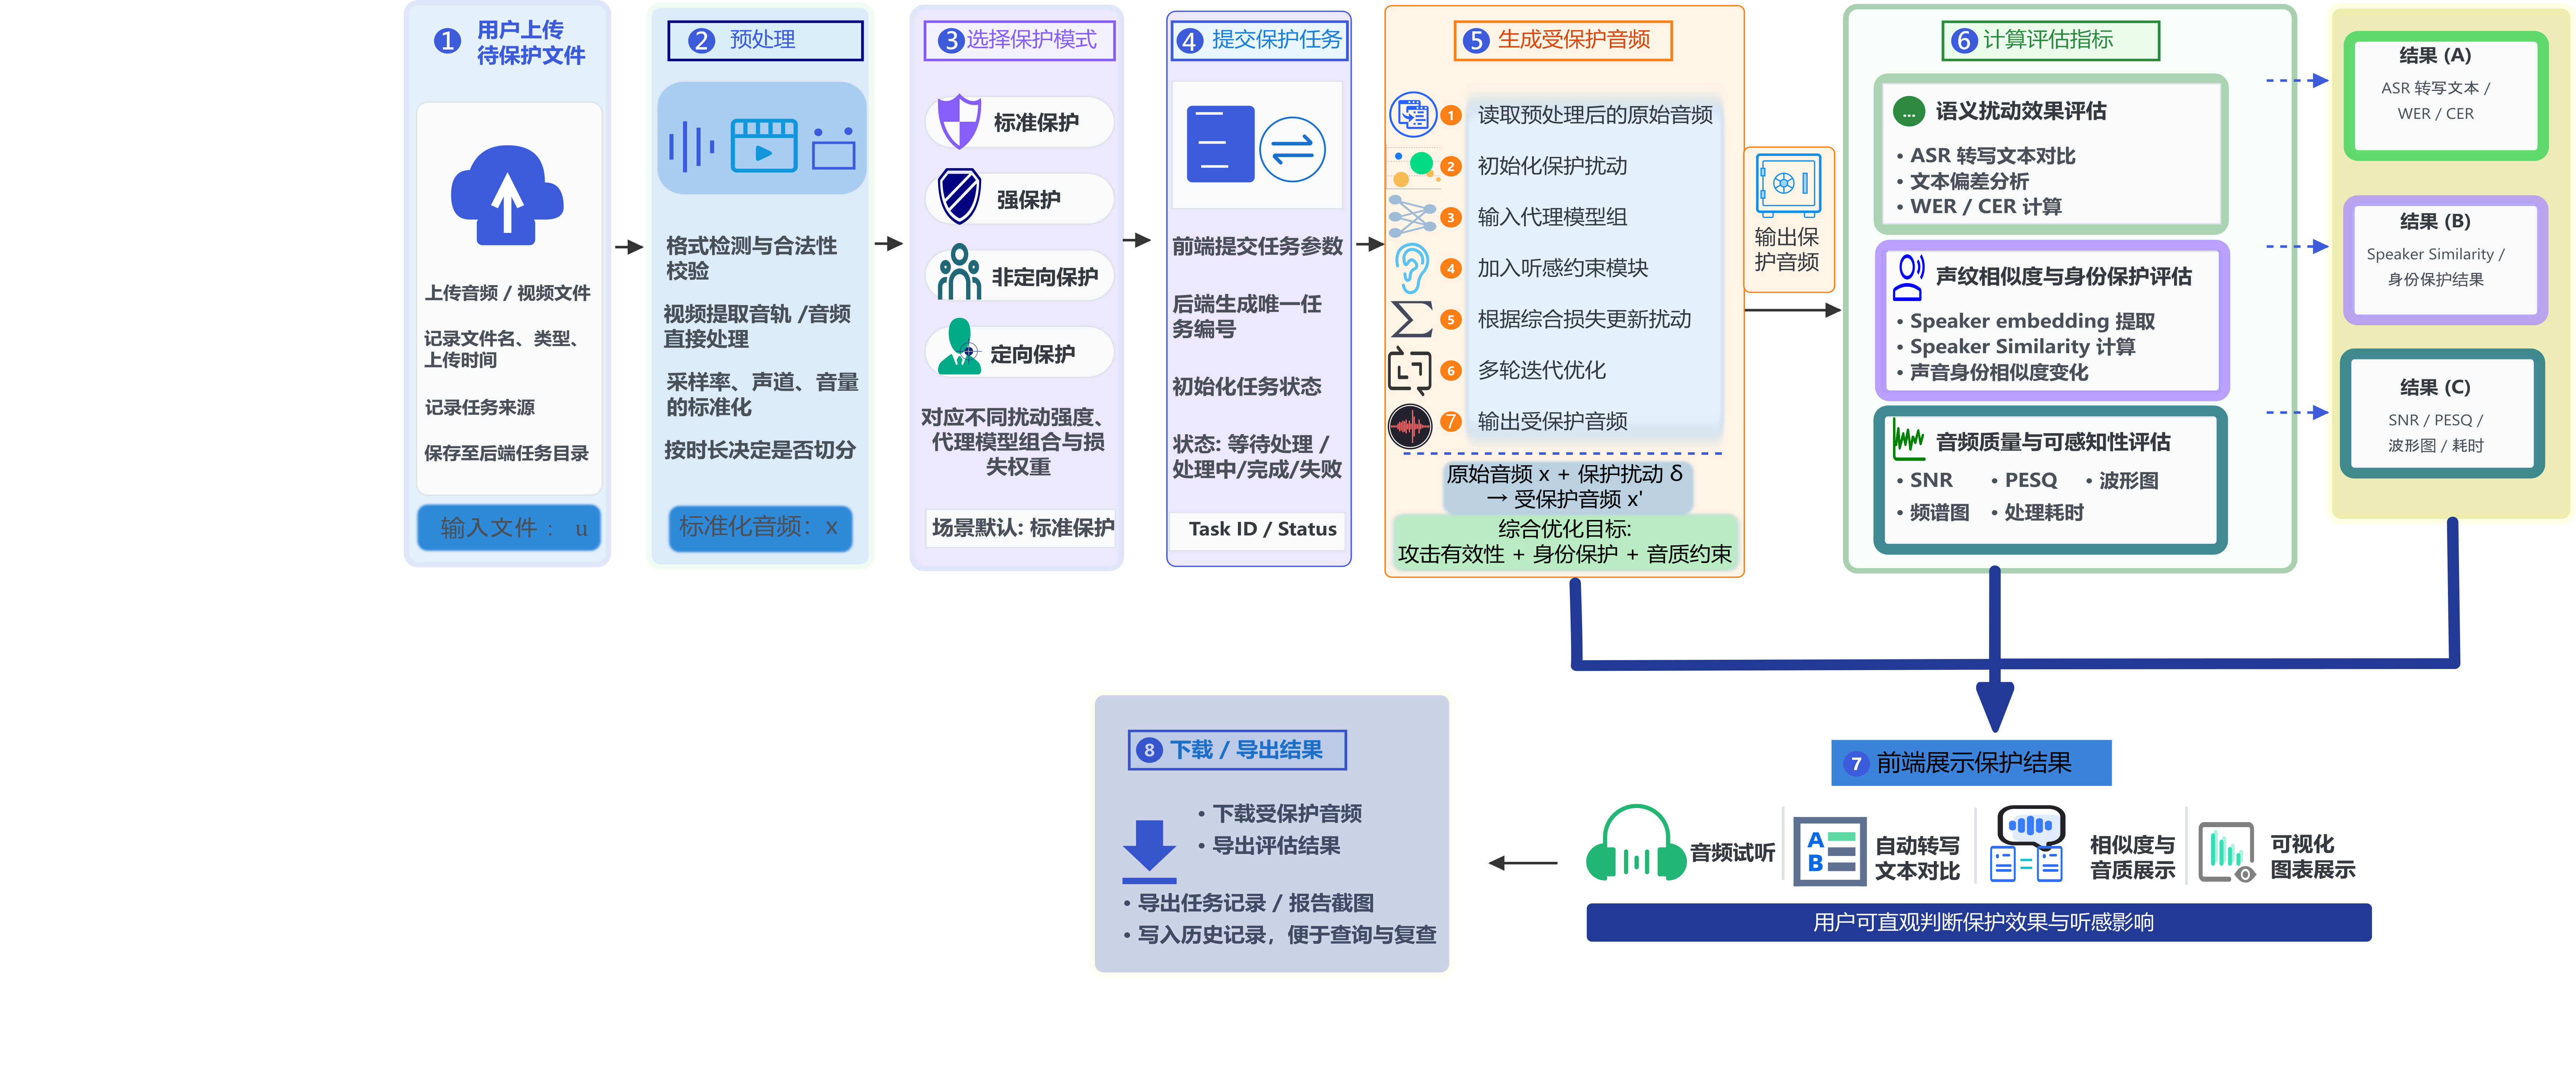
\includegraphics[width=\textwidth,height=0.72\textheight,keepaspectratio]{figures/image16.png}
  \caption{用户视角的系统工作流程}
  \label{fig:3-2}
\end{figure}

第一步，用户上传待保护文件。用户可以在网页端上传音频或视频文件，系统记录文件名、文件类型、上传时间和任务来源，并将文件保存到后端任务目录中。

第二步，系统进行预处理。后端对上传文件进行格式检测和合法性校验。如果用户上传的是视频文件，系统先抽取其中的音轨；如果用户上传的是音频文件，系统直接进入格式标准化流程。随后，系统统一采样率、声道数和音量，并根据音频时长决定是否进行切分。

第三步，用户选择保护模式。系统可提供标准保护、强保护、非定向保护和定向保护等模式。不同模式对应不同扰动强度、代理模型组合和损失权重设置。对于普通用户，系统可默认采用标准保护模式；对于演示或高风险场景，可选择更强的保护配置。

第四步，用户提交保护任务。前端将任务参数发送给后端，后端为该任务生成唯一任务编号，并初始化任务状态。任务状态通常包括等待处理、处理中、处理完成和处理失败等。

第五步，系统生成受保护音频。主动保护生成模块读取预处理后的原始音频，初始化保护扰动，并将当前音频输入代理模型组和听感约束模块。系统根据综合损失更新保护扰动，经过多轮迭代后输出受保护音频。

第六步，系统计算评估指标。后端将原始音频和受保护音频同时输入评估模块，计算
ASR 转写差异、WER /
CER、声音身份相似度、SNR、PESQ、波形图、频谱图和处理耗时等结果。

第七步，前端展示保护结果。结果页面展示原始音频与受保护音频的试听控件、自动转写文本对比、声音身份相似度变化、音频质量指标和可视化图表，使用户可以直观判断保护效果和听感影响。

第八步，用户下载或导出结果。用户可以下载受保护音频，也可以导出评估结果、任务记录或报告截图。系统同时将任务相关信息写入历史记录，便于后续查询和复查。

上述流程使 V-Guard
形成从文件输入到保护输出的完整闭环。用户只需完成少量交互操作，系统即可自动完成音频标准化、主动防护生成、效果评估和结果展示。

\subsection{系统功能模块}\label{ux7cfbux7edfux529fux80fdux6a21ux5757}

根据系统工作流程，V-Guard
可进一步划分为六个主要功能模块：音频/视频接入与预处理模块、主动保护生成模块、ASR
转写对比模块、声音身份相似度评估模块、音频质量评估模块以及 Web
交互与结果导出模块。


\begin{figure}[htbp]
  \centering
  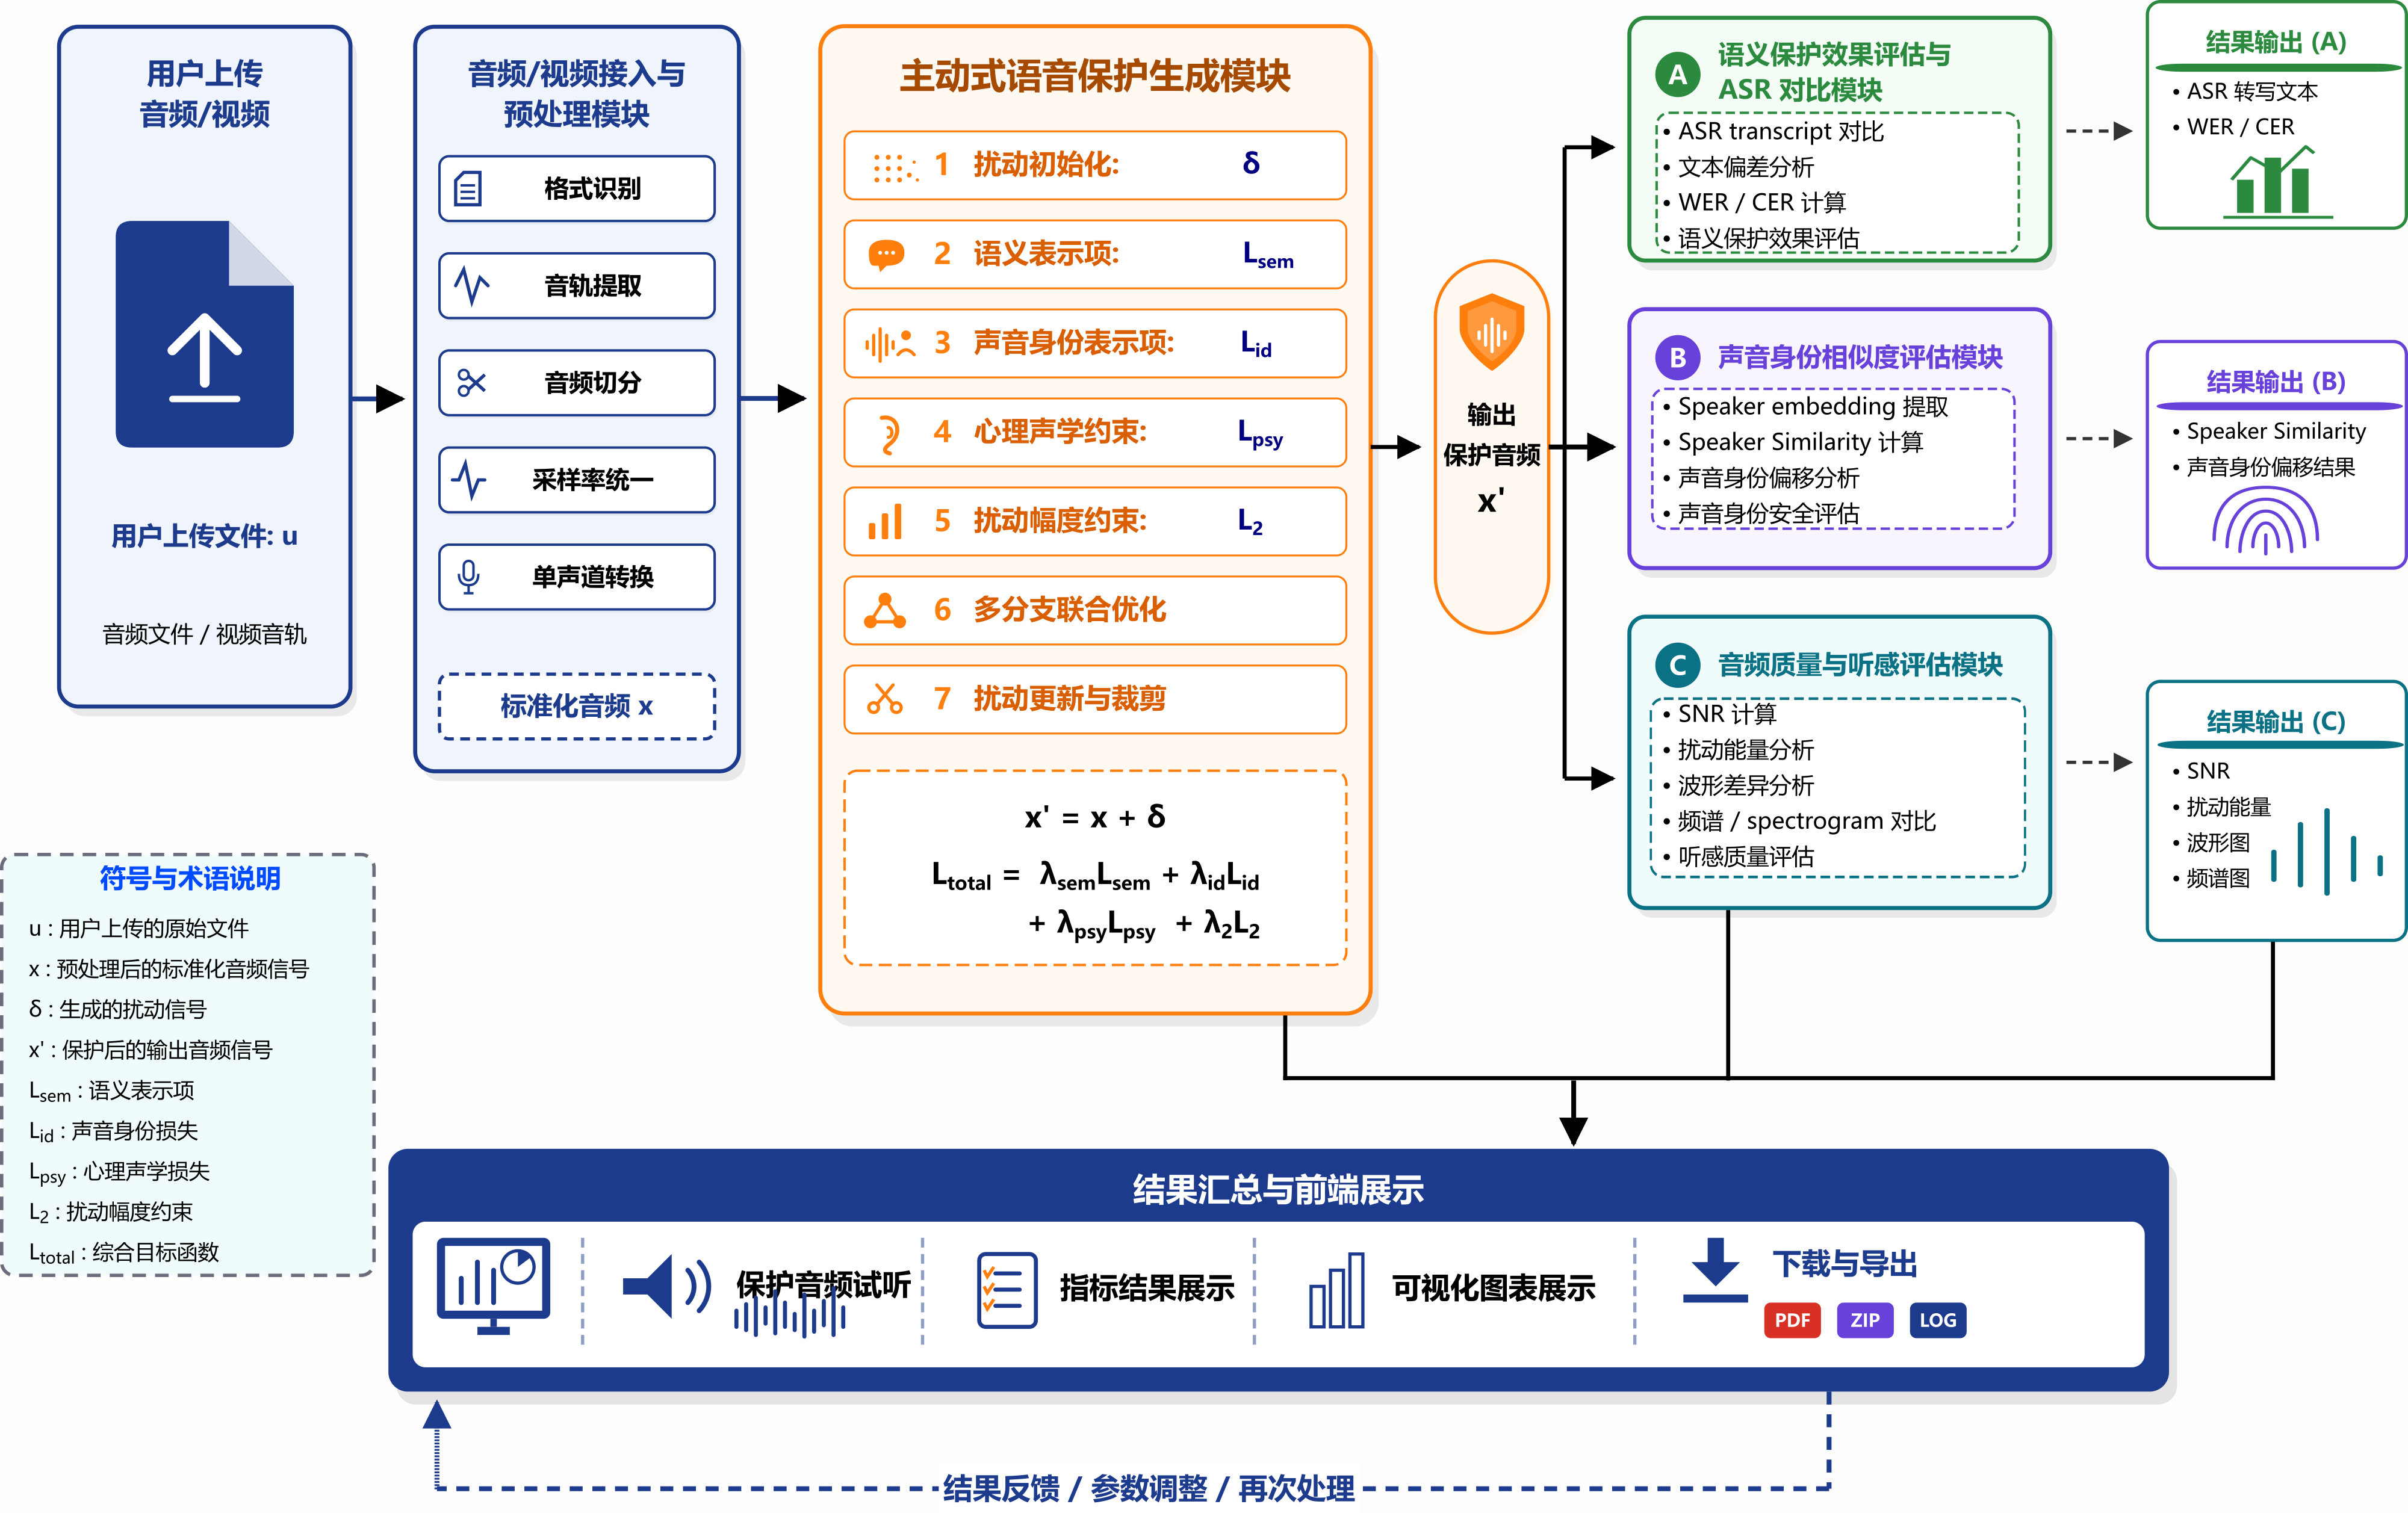
\includegraphics[width=\textwidth,height=0.72\textheight,keepaspectratio]{figures/image17.png}
  \caption{系统功能模块调用示意图}
  \label{fig:3-3}
\end{figure}

音频/视频接入与预处理模块负责接收用户上传文件，并将其转换为后续算法可处理的标准音频格式。该模块屏蔽不同格式、采样率、声道数、音量大小和音频时长带来的差异，是整个系统的数据入口。

主动保护生成模块负责根据原始音频生成受保护音频。该模块调用语义表示链路保护、声音身份特征链路保护、听感约束和扰动幅度控制等算法组件，在原始音频上生成保护扰动。

ASR
转写对比模块负责分析保护前后音频在机器语义理解层面的变化。该模块分别对原始音频和受保护音频进行自动转写，并计算
WER / CER 等文本差异指标，用于观察保护音频对语义表示链路的影响。

声音身份相似度评估模块负责分析保护前后音频在机器声音身份表示层面的变化。该模块提取原始音频和受保护音频的说话人嵌入或声音身份表示，并计算说话人相似度，用于评估系统是否降低机器对原始说话人身份信息的稳定提取能力。

音频质量评估模块负责分析保护扰动是否明显影响正常听感。该模块计算
SNR、PESQ
等指标，并生成波形图和频谱图，辅助判断受保护音频是否仍然具备正常播放、发布和展示价值。

Web
交互与结果导出模块负责将上述功能封装为用户可操作的网页流程。该模块提供文件上传、保护模式选择、任务提交、任务状态查看、结果展示、历史记录和文件下载等功能，使底层主动防护算法能够以完整作品形式呈现。

\section{系统核心技术}\label{ux7cfbux7edfux6838ux5fc3ux6280ux672f}

第三章的重点是系统实现，但主动保护生成仍然是 V-Guard
的核心技术基础。因此，本节只保留必要的算法流程和关键公式，说明系统如何从原始音频生成受保护音频。需要说明的是，本作品的核心算法并非直接照搬原始
E2E-VGuard 中以 ASR
目标文本为中心的发音扰动形式，而是在其声音身份保护与心理声学约束思想基础上，引入面向语义表示与语音分词器前端的语义扰动目标。系统最终采用``语义表示保护、声音身份保护、心理声学约束和扰动幅度控制''共同优化的方式生成受保护音频。更详细的语音表示、语音分词器、对抗扰动和听感评价背景已在第二章说明。

\subsection{核心算法流程}\label{ux6838ux5fc3ux7b97ux6cd5ux6d41ux7a0b}

设用户上传并经过预处理后的原始音频为 \(x\)，系统生成的保护扰动为
\(\delta\)，最终输出的受保护音频为 \(x'\)，则三者关系为：

\[x' = x + \delta\]

主动防护的核心矛盾在于：\(\delta\)
不能过大，否则会破坏用户正常收听和发布音频的需求；但 \(\delta\)
又必须足以影响机器模型对语音的表示提取，否则无法降低未授权语音克隆系统对原始声音资产的利用能力。

系统在每轮迭代中将当前受保护音频输入语义代理模型组、声音身份代理模型组和听感约束模块，并计算综合目标。综合目标主要由四部分组成：语义表示损失、声音身份损失、心理声学听感约束和扰动幅度约束。其中，语义表示损失记为
\(\mathcal{L}_{sem}\)，用于推动受保护音频在语义编码器、ASR encoder
或语音分词器前端表示空间中偏离原始音频，从而影响机器对``说了什么''的稳定建模；声音身份损失记为
\(\mathcal{L}_{id}\)，用于推动受保护音频在说话人嵌入、音色编码器或风格编码器表示空间中偏离原始说话人，从而影响机器对``是谁在说、怎么说''的稳定提取；心理声学约束记为
\(\mathcal{L}_{psy}\)，用于控制扰动在时频空间中的可感知性；扰动幅度约束记为
\(\mathcal{L}_{2}\)
，用于限制保护音频与原始音频之间的整体数值差异。综合目标可概括写为：

\[\mathcal{L}(x')\  = \ \lambda_{sem}\mathcal{L}_{sem}(x,\ x')\  + \ \lambda_{id}\mathcal{L}_{id}(x,x')\  + \ \lambda_{psy}\mathcal{L}_{psy}(x,\delta) + \ \lambda_{2}\mathcal{L}_{2}(\delta)\]

其中，\(\mathcal{L}_{sem}\) 表示语义表示项，\(\mathcal{L}_{id}\ \)
表示声音身份表示项，\(\mathcal{L}_{psy}\) 表示心理声学听感约束项，\(\mathcal{L}_{2}\)
表示扰动幅度项；\(\lambda_{sem}\)、\(\lambda_{id}\)、\(\lambda_{psy}\)
和 \(\lambda_{2}\)
分别表示各项权重，用于控制不同目标在优化过程中的相对重要程度。

在优化过程中，系统不重新训练 ASR
模型、语音合成模型、语音分词器或说话人识别模型，而是在冻结语义代理模型组和声音身份代理模型组参数的条件下，仅优化输入侧保护扰动
\(\delta\)。系统根据综合损失 \(\mathcal{L}\ \)对扰动 \(\delta\)
求梯度，并采用投影梯度下降（Projected Gradient
Descent，PGD）思想更新扰动\textsuperscript{{[}51{]}}。每轮更新后，系统将扰动投影回允许范围内，并将受保护音频裁剪到合法波形区间，避免扰动在迭代中无限累积。更新后，系统将扰动投影回允许范围内，并将受保护音频裁剪到合法波形区间。单轮更新可概括为：

\[\delta^{(k + 1)}\  = \ {Proj}_{\delta}\ \  \leq \ \epsilon(\delta^{(k)}\  - \ \alpha\  \bullet \ sign(\nabla_{\delta}\mathcal{L}))\]

\[{x'}^{\ (k\  + \ 1)}\  = \ {Clip}_{\lbrack - 1.1\rbrack}(x\  + \ \delta^{(k + 1)})\]

其中，\(k\) 表示迭代轮数，\(\alpha\) 表示单步更新幅度，\(\epsilon\)
表示扰动幅度上限，\(Proj\) 表示扰动投影操作，\(Clip\)
表示波形裁剪操作。通过多轮迭代，系统逐步得到满足幅度约束和听感约束的受保护音频。


\begin{figure}[htbp]
  \centering
  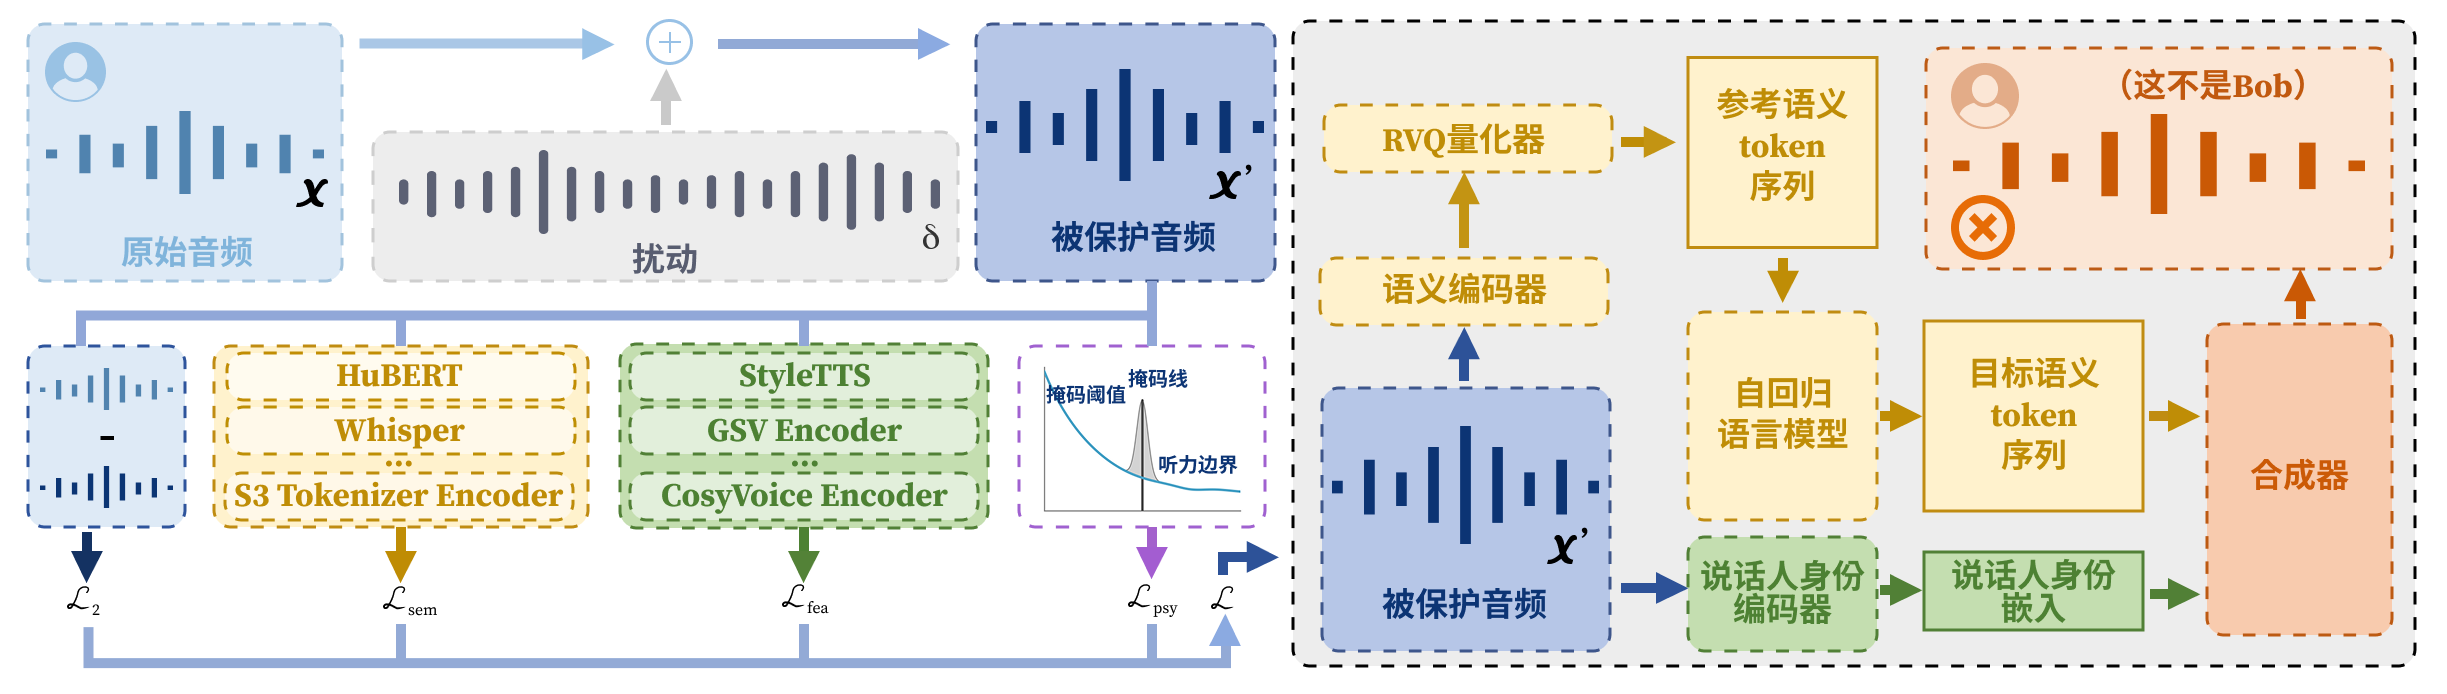
\includegraphics[width=\textwidth,height=0.72\textheight,keepaspectratio]{figures/image18.png}
  \caption{主动保护生成流程图}
  \label{fig:3-4}
\end{figure}

具体的算法执行步骤如下所示：


\begin{algorithm}[H]
\caption{V-Guard 主动保护扰动生成算法}
\label{alg:vguard}
\small
\begin{algorithmic}[1]
    \Inputs 原始音频 $x$，最大迭代步数 $N_{iter}$，保护模式 $m \in \{\mathrm{targeted},\mathrm{untargeted}\}$。
    \Parameters 最大扰动幅度 $\epsilon$，损失权重 $\lambda_{sem}, \lambda_{id}, \lambda_{psy}, \lambda_{2}$，更新步长 $\eta$。
    \Output 受保护音频 $x'$。

    \State $\delta \gets \mathrm{Uniform}(-\epsilon, \epsilon)$；
    \State $x' \gets \mathrm{Clamp}(x + \delta, -1.0, 1.0)$；
    \State $Z_{x}^{sem} \gets \mathcal{F}_{sem}(x)$，$Z_{x}^{id} \gets \mathcal{F}_{id}(x)$；
    \State $\Theta_{x}, P_{x} \gets \mathrm{Masker}(x)$；
    \If{$m = \mathrm{targeted}$}
        \State $x_{t} \gets \mathrm{SelectTargetAudio}(x)$；
        \State $Z_{t}^{id} \gets \mathcal{F}_{id}(x_{t})$；
    \EndIf

    \For{$i \gets 1$ \textbf{to} $N_{iter}$}
        \State $Z_{x'}^{sem} \gets \mathcal{F}_{sem}(x')$，$Z_{x'}^{id} \gets \mathcal{F}_{id}(x')$；
        \If{$m = \mathrm{targeted}$}
            \State $\mathcal{L}_{id} \gets -\mathrm{Sim}_{id}\!\left(Z_{t}^{id}, Z_{x'}^{id}\right)$；
        \Else
            \State $\mathcal{L}_{id} \gets \mathrm{Sim}_{id}\!\left(Z_{x}^{id}, Z_{x'}^{id}\right)$；
        \EndIf
        \State $\mathcal{L}_{sem} \gets \mathrm{Sim}_{sem}\!\left(Z_{x}^{sem}, Z_{x'}^{sem}\right)$；
        \State $\mathcal{L}_{psy} \gets \mathrm{PsyLoss}\!\left(\delta, \Theta_{x}, P_{x}\right)$；
        \State $\mathcal{L}_{2} \gets \lVert \delta \rVert_{2}$；
        \State $\mathcal{L} \gets \lambda_{sem}\mathcal{L}_{sem}+\lambda_{id}\mathcal{L}_{id}+\lambda_{psy}\mathcal{L}_{psy}+\lambda_{2}\mathcal{L}_{2}$；
        \State $\delta \gets \mathrm{Clamp}\!\left(\delta-\eta\cdot\mathrm{sign}\left(\nabla_{\delta}\mathcal{L}\right), -\epsilon, \epsilon\right)$；
        \State $x' \gets \mathrm{Clamp}(x+\delta, -1.0, 1.0)$；
    \EndFor
    \State \Return $x'$；
\end{algorithmic}
\end{algorithm}

\subsection{面向语义表示链路的保护}\label{ux9762ux5411ux8bedux4e49ux8868ux793aux94feux8defux7684ux4fddux62a4}

语义表示链路保护面向机器对``说了什么''的理解过程。语音克隆系统在训练、微调、自动标注或大模型语音合成场景中，可能需要从参考音频中提取语音内容、发音单元、文本转写、语义
token
或文本---发音对齐关系。如果攻击者只有公开语音而没有人工标注文本，ASR
系统可能被用于生成转写文本；如果攻击者使用基于语音分词器或大语言模型的语音系统，参考音频还可能先被编码为连续语义表示或离散语音
token。因此，本作品不把语义保护简单等同于攻击某一个 ASR
最终文本输出，而是优先影响语义编码器、ASR encoder
和语音分词器前端的中间表示。

在系统实现中，V-Guard 不把优化目标限定为某一个 ASR
系统的最终文本输出。最终文本通常已经经过声学编码器、解码器、语言模型、分词规则和文本后处理等多个环节，直接对最终转写结果构造损失不仅反向优化不稳定，也容易过度依赖某一个具体
ASR 系统的解码策略。相比之下，ASR encoder、语义 encoder 或语音分词器
encoder
的中间表示更靠近语音模型前端，能够更直接地反映机器对语音内容、发音结构和语义单元的编码过程。因此，本作品将语义保护目标定义为
\(\mathcal{L}_{sem}\)，优先在多个语义代理编码器的表示空间中推动受保护音频偏离原始音频。ASR
转写差异、WER 和 CER
主要作为前端可展示的语义保护效果指标，而不是当前优化过程的唯一目标。

从模型类型看，语义表示链路可以分为连续表示路径和离散 token
路径。连续表示路径主要对应 ASR
编码器、自监督语音表示模型和语义编码器等模块，它们将输入波形转换为连续隐藏向量或逐帧表示。离散
token 路径则主要对应语音分词器，其通常先通过 encoder
得到连续语音表示，再通过量化器将连续表示映射为离散语音
token。现代语音系统既可能通过 ASR
模型获得文本结果，也可能通过语音分词器将连续语音表示转换为离散语音
token，再交由后续语音大模型建模\textsuperscript{{[}31,37,40{]}}。WavLM
等全栈语音预训练模型也说明，语音表示中往往同时包含说话内容、说话人身份和副语言信息，因此从中间表示层面进行保护，比只观察最终文本输出更适合覆盖多类语音处理流程\textsuperscript{{[}39{]}}。

为了降低对单一代理模型的依赖，系统将语义代理模型组织为一个代理模型组，而不是只使用单个
\(E_{sem}\)。设语义代理模型组为：

\[\mathcal{E}_{sem}\  = \ E_{sem}^{(1)},\ E_{sem}^{(2)},\ \ldots,\ E_{sem}^{(M)}\]

其中，\(E_{sem}^{(i)}\) 表示第 \(i\) 个语义代理模型，\(M\)
表示语义代理模型数量。该集合可以包含三类模型：第一类是 ASR
encoder，例如用于语音转写任务的声学编码器，它主要刻画语音内容和发音结构；第二类是自监督语音表示模型或语义
encoder，例如 wav2vec 2.0、HuBERT、WavLM
一类模型中的语音表示前端，它主要刻画语音信号中的通用语义和声学信息；第三类是语音分词器
encoder，例如 SpeechTokenizer
等模型中的连续表示前端，它先提取连续语音表示，再进入后续量化模块形成离散语音
token。不同模型的训练目标、结构和输出维度可能不同，但它们都从某个角度刻画机器对语音内容、发音结构或语义
token 的理解过程。

对于第 \(i\) 个语义代理模型，系统分别提取原始音频 \(x\) 和受保护音频
\(x'\)
的语义表示。由于不同模型输出可能是逐帧序列，也可能是分层隐藏表示，系统可将其整理为可比较的表示向量：

\[h_{sem}^{(i)}\ \  = \ E_{sem}^{(i)}(x)\]

\[{h_{sem}^{(i)}}'\  = \ E_{sem}^{(i)}(x'\ )\]

对于单个语义代理模型，语义表示相似度损失可写为：

\[\mathcal{L}_{sem}^{(i)}(x,\ x'\ )\ \  = \ Sim(h_{sem}^{(i)}\ ,\ {h_{sem}^{(i)}}'\ )\  = \ Sim(E_{sem}^{(i)}(x)\ ,\ E_{sem}^{(i)}(x'\ ))\ \]

其中，\(Sim\)(\(\bullet , \bullet\))
可表示余弦相似度或其他向量相似度度量。若 \(\mathcal{L}_{sem}^{(i)}\ \)
较高，说明第 \(i\)
个语义代理模型仍将受保护音频视为与原始音频相近的语义输入；若该值下降，则说明保护扰动已经使该模型中的语义表示发生偏移。

在多代理场景下，系统对多个语义代理模型的损失进行加权集成，得到整体语义表示项：

\[\mathcal{L}_{sem}\  = \ \sum_{i\  = \ 1}^{M}{w_{sem}^{(i)}\mathcal{L}_{sem}^{(i)}}\]

\[\sum_{i\  = \ 1}^{M}w_{sem}^{(i)}\  = \ 1,\ w_{sem}^{(i)}\  > \ 0\]

其中，\(w_{sem}^{(i)}\) 表示第 \(i\)
个语义代理模型的权重。权重可根据模型重要性、计算成本、输出稳定性和任务相关性设定。该集成不是简单投票，而是在损失函数层面对多个语义表示空间进行融合。对抗样本迁移性研究表明，基于多个代理模型生成扰动有助于提升黑盒场景下的迁移能力\textsuperscript{{[}52{]}}。因此，V-Guard
采用语义代理模型组，可以降低保护扰动对单一 ASR
或单一语音分词器的依赖，使扰动更关注多类语音系统共同依赖的前端语义表示。

对于连续表示型语音模型，降低 \(\mathcal{L}_{sem}^{(i)}\ \)会直接推动受保护音频在
ASR encoder、自监督语音 encoder 或语义 encoder
的连续表示空间中偏离原始音频。这种偏移可能影响后续文本转写、发音单元建模或文本---语音对齐结果。对于包含语音分词器的模型，保护扰动首先影响的仍然是语音分词器
encoder
输出的连续表示；当连续表示靠近量化边界时，较小的表示偏移可能改变后续量化器选择的离散语音
token，并且造成更大的语义偏移。也就是说，离散 token
的变化不是凭空产生，而是由前端连续表示偏移进一步传导到量化结果。SpeechTokenizer
等工作表明，语音 token 可以区分语义 token 与声学
token，并通过量化结构连接连续语音表示和离散 token
序列\textsuperscript{{[}31{]}}。相关语音分词器安全研究进一步指出，语音分词器位于连续语音表示与离散
token 建模之间，针对语音分词器 encoder 的语义表示扰动可能引起 token
级变化，并进一步影响下游 ASR
或语音大模型理解\textsuperscript{{[}41{]}}；离散音频 token
的综述性研究也说明，离散 token
已成为语音理解、语音生成和音频大模型中的重要中间表示\textsuperscript{{[}33{]}}。因此，语义表示项
的设计既能覆盖连续表示型语音理解流程，也能兼容基于语音分词器的新型语音大模型前端。

需要注意的是，系统并不假设每一次连续表示偏移都会导致大规模离散 token
跳变。离散 token
是否变化，取决于语音分词器的量化边界、码本结构、模型鲁棒性和输入扰动位置。保护扰动首先作用于连续语音表示，在部分包含量化模块的系统中，这种连续表示偏移可能进一步引起离散语音
token 的变化，从而影响后续语言模型或生成模型对参考音频的建模。

在系统展示层面，语义表示链路保护的结果通过 ASR
转写对比、词错误率（WER，Word Error Rate）和字符错误率（CER，Character
Error Rate）等指标呈现。需要注意的是，ASR
文本对比主要是用户可观察的结果展示，不一定是系统优化的唯一目标。系统更关注的是保护音频是否在机器语义表示链路中发生偏移，并通过最终转写差异辅助用户理解这种偏移的可见效果。

\subsection{面向声音身份特征链路的保护}\label{ux9762ux5411ux58f0ux97f3ux8eabux4efdux7279ux5f81ux94feux8defux7684ux4fddux62a4}

声音身份特征链路保护面向机器对``是谁在说、怎么说''的提取过程。语音克隆系统即使已经获得攻击者输入的目标文本，仍然需要从参考音频中提取说话人身份、音色、韵律、风格和声学条件等声音身份信息。如果受保护音频能够降低这些表示与原始说话人之间的稳定对应关系，就可能削弱后续克隆系统对目标声音的复刻能力。声音身份损失
\(\mathcal{L}_{id}\)
面向机器对说话人身份、音色、韵律、风格和声学条件的提取过程。系统通过说话人编码器、TTS
音色编码器、风格编码器或声学特征提取器等身份代理模型，提取原始音频与受保护音频的声音身份表示，并通过降低二者在身份表示空间中的相似度，使机器更难稳定提取原始说话人的声音条件。

在系统实现中，V-Guard
通过说话人编码器、声音身份编码器、风格编码器或声学特征提取器等代理模型，近似语音克隆系统对参考音频中声音身份信息的提取过程。说话人识别领域中的
x-vector、ECAPA-TDNN 和 CAM++
等工作已经证明，将不同长度语音映射为固定维度说话人嵌入，是进行说话人验证和相似度度量的有效方式\textsuperscript{{[}42-45{]}}。主动语音防护和语音转换防护相关工作也表明，通过在待保护语音中加入不可感知扰动或不可学习扰动，可以降低模型对原始说话人特征的稳定利用能力\textsuperscript{{[}19-23{]}}。

与语义表示链路类似，系统不假设某一个声音身份代理模型能够完整代表所有攻击模型。不同攻击者可能使用不同说话人编码器、不同
TTS
后验编码器、不同风格编码器或不同声学条件提取器。为了降低对单一声纹模型的依赖，系统将声音身份代理模型组织为代理模型组：

\[\mathcal{E}_{id}\  = \ E_{id}^{(1)},\ E_{id}^{(2)},\ \ldots,\ E_{id}^{(K)}\]

其中，\(E_{id}^{(j)}\) 表示第 \(j\) 个声音身份代理模型，\(K\)
表示声音身份代理模型数量。该集合可以包含四类模型：第一类是说话人验证模型，例如
x-vector、ECAPA-TDNN 等模型，它们主要提取说话人身份嵌入；第二类是 TTS
或语音克隆系统中的说话人编码器，它们通常将参考音频转换为后续合成模块使用的说话人条件；第三类是风格编码器或韵律编码器，它们主要刻画说话方式、节奏、语速、情绪和风格信息；第四类是传统声学特征提取器，例如梅尔频率倒谱系数（MFCC，Mel-Frequency
Cepstral
Coefficients）等，用于从较基础的声学层面描述语音频谱结构。它们不一定输出同一种特征，但都从某个角度描述参考音频中的声音身份条件。对于第
\(j\)
个声音身份代理模型，系统分别提取原始音频和受保护音频的声音身份表示：

\[h_{id}^{(j)}\ \  = \ E_{id}^{(j)}(x)\]

\[{h_{id}^{(j)}}'\  = \ E_{id}^{(j)}(x'\ )\]

在非定向保护模式下，系统希望受保护音频远离原始说话人的声音身份表示。对于单个声音身份代理模型，其损失可写为：

\[\mathcal{L}_{id}^{(j)}\  = \ Sim(h_{id}^{(j)}\ ,\ {h_{id}^{(j)}}'\ )\]

在多代理模型组中，系统对所有声音身份代理模型的损失进行加权集成：

\[\mathcal{L}_{id}^{untargeted}\  = \ \sum_{j\  = \ 1}^{K}{w_{id}^{(j)}\mathcal{L}_{id}^{(j)}}\  + \ w_{m}Sim(M(x),\ M(x'\ ))\]

\[\sum_{j\  = \ 1}^{K}w_{id}^{(j)}\  = \ 1,\ w_{id}^{(j)}\  > \ 0\]

其中，\(w_{id}^{(j)}\) 表示第 \(j\)
个声音身份代理模型的权重，\(M( \bullet )\)
表示梅尔频率倒谱系数（MFCC，Mel-Frequency Cepstral
Coefficients）或其他传统声学特征提取函数，\(w_{m}\)
表示传统声学特征项的权重。优化过程中，系统通过降低\(\mathcal{L}_{id}^{untargeted}\)
，使受保护音频在多个声音身份表示空间中同时远离原始音频；同时，通过降低
\(Sim(M(x),\ M(x'\ ))\)，使受保护音频在传统声学特征空间中也不再与原始音频保持过高相似度。这样即使攻击者使用受保护音频作为参考语音，模型也更难稳定提取原始说话人的身份条件。

在定向保护模式下，系统还可以引入目标参考音频
\(x_{t}\)，使受保护音频在机器表示中远离原始说话人，同时朝指定目标声音身份表示靠近。设第
\(j\) 个代理模型中目标参考音频的声音身份表示为：

\[h_{target\_ id}^{(j)}\  = \ E_{id}^{(j)}(x_{t})\]

则定向保护模式下的声音身份损失可写为：

\[\mathcal{L}_{id}^{targeted}\  = \  - \sum_{j}^{K}{\ w_{id}^{(j)}Sim(h_{target\_ id}^{(j)}\ ,\ {h_{id}^{(j)}}'\ )\rbrack}\  - \ \ w_{m}Sim(M(x_{t}),\ M(x'\ ))\]

该式中的负号表示，优化器在最小化 \(\mathcal{L}_{id}^{targeted}\)
时，会提高受保护音频与目标参考音频在声音身份代理模型空间中的相似度；同时，也会提高受保护音频与目标参考音频在传统声学特征空间中的相似度。因此，定向保护模式的核心作用不是简单地让受保护音频随机远离原始说话人，而是将机器提取到的声音身份表示引导到指定目标方向。定向模式适合安全演示或特定保护策略；普通用户场景中可默认使用非定向保护模式，以降低系统使用复杂度。非定向与定向的声音身份混淆流程如下图所示：


\begin{figure}[htbp]
  \centering
  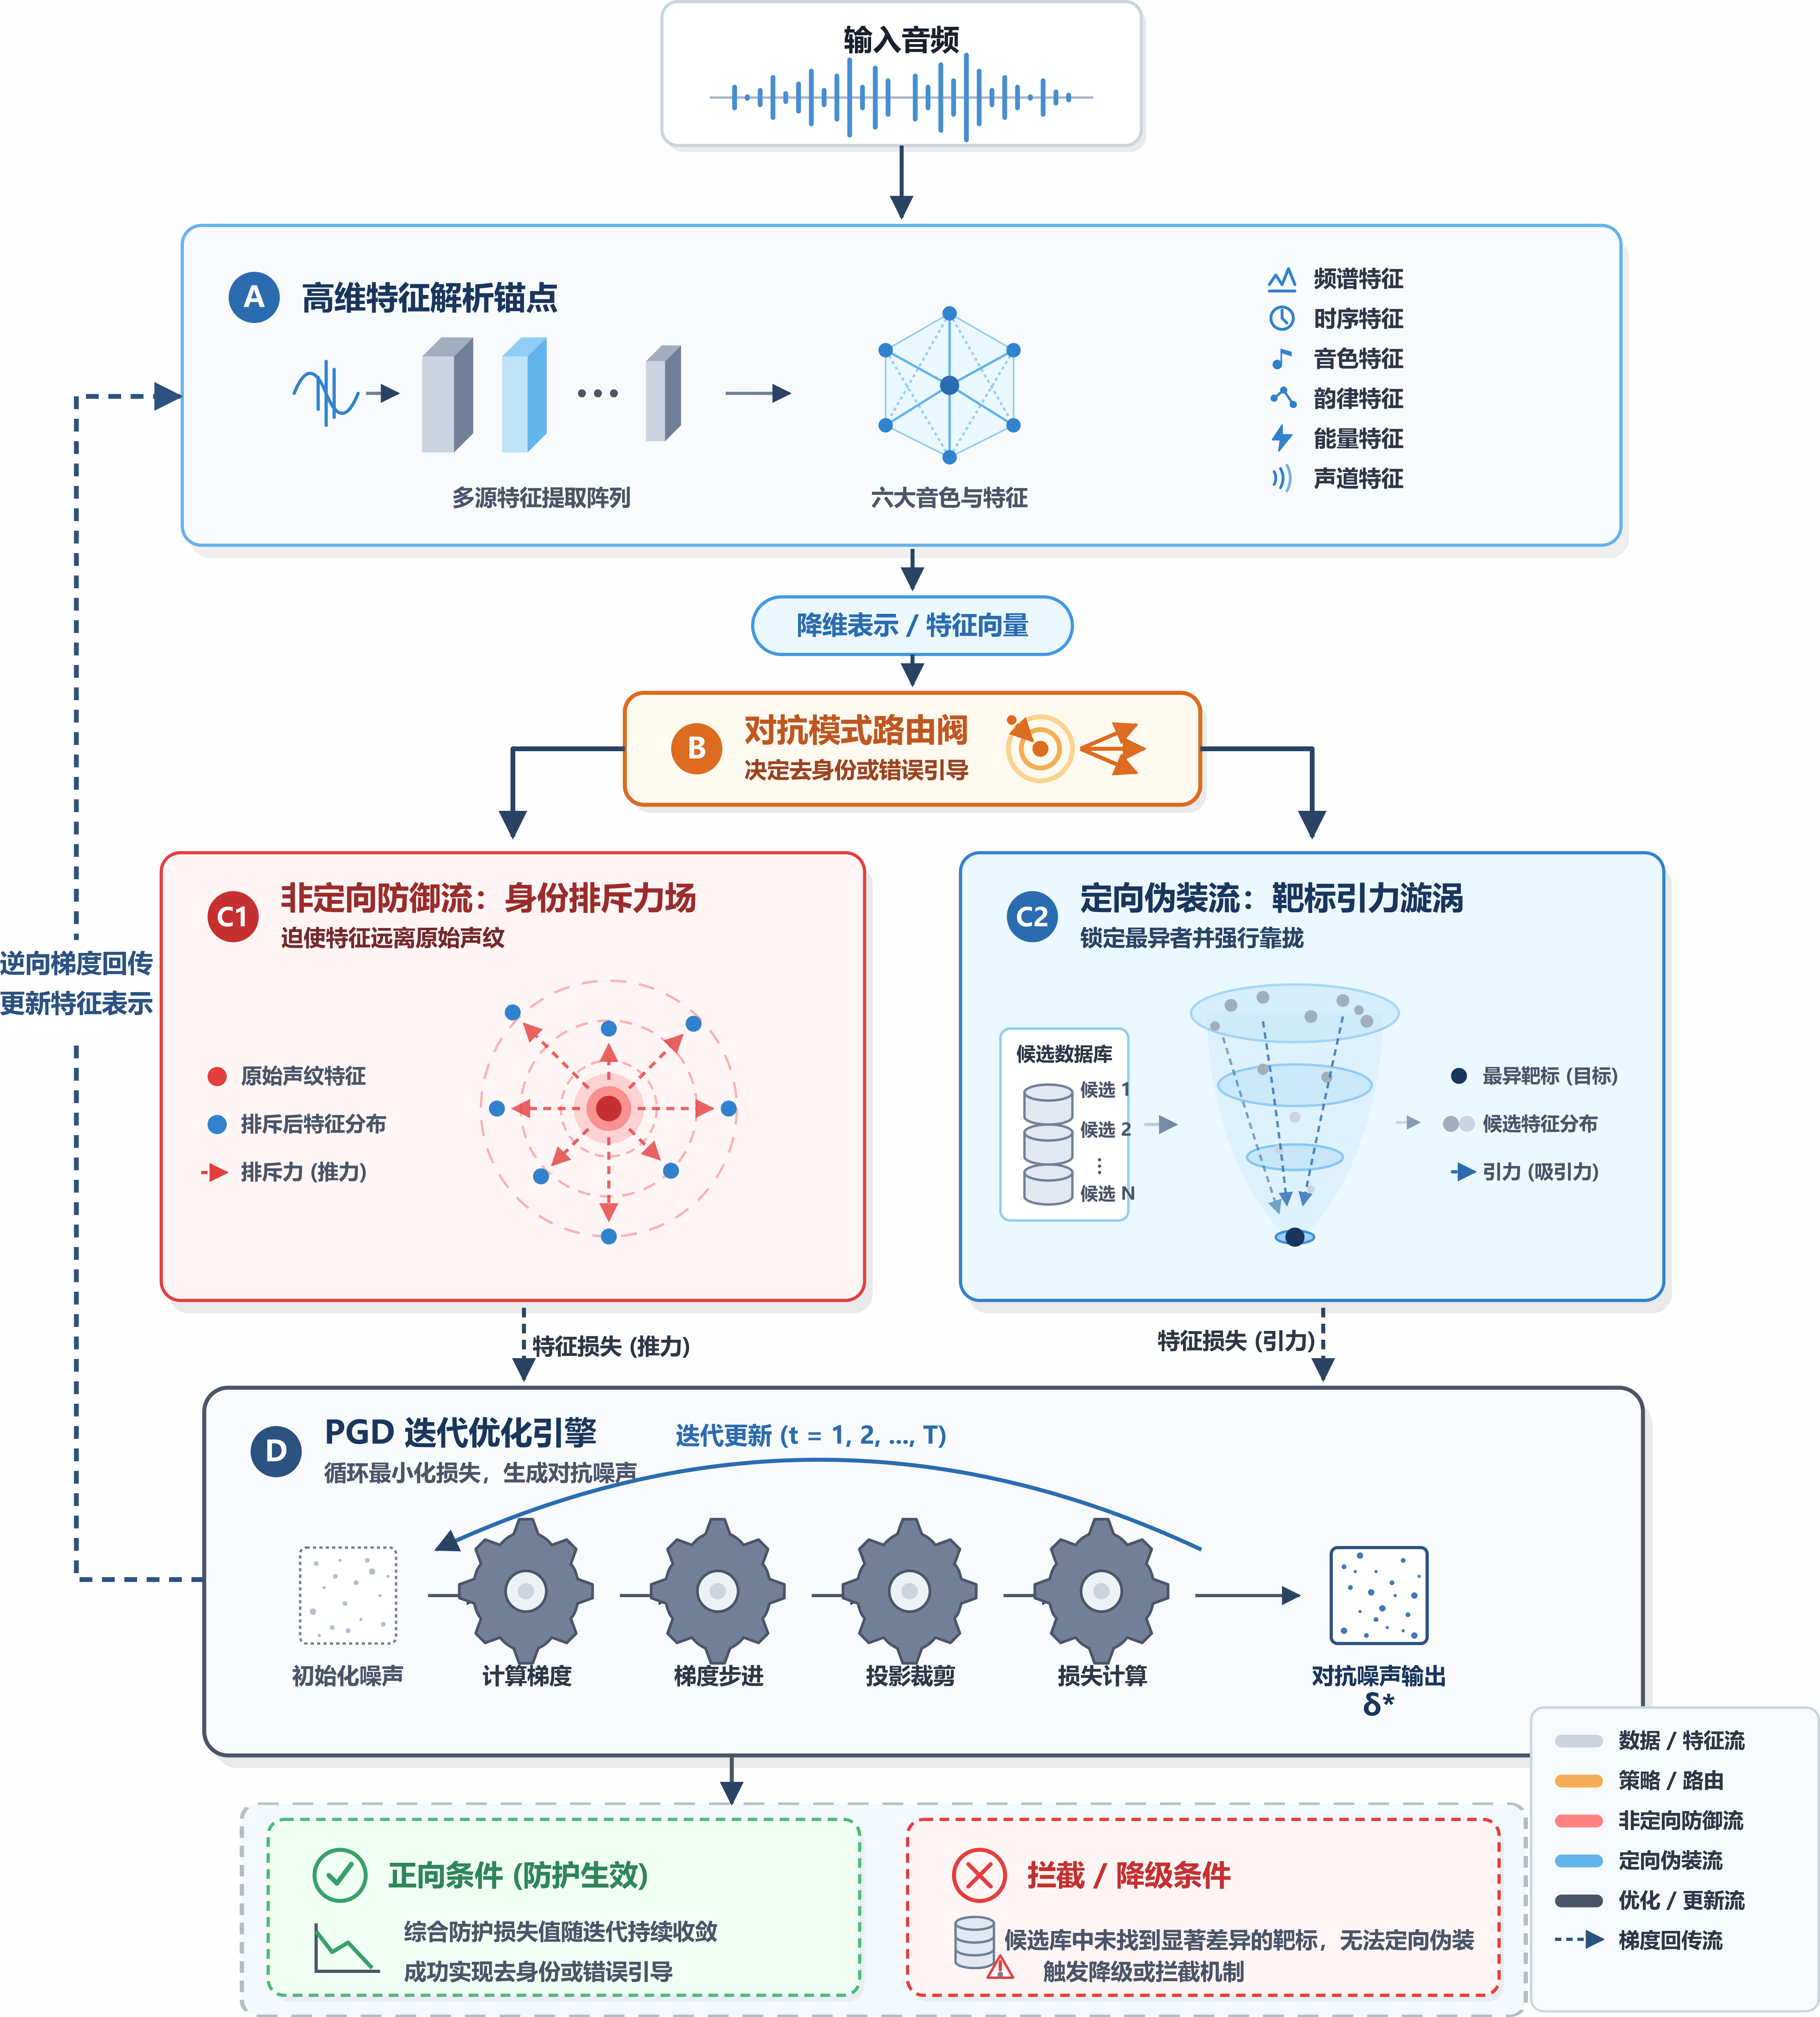
\includegraphics[width=\textwidth,height=0.72\textheight,keepaspectratio]{figures/image20.png}
  \caption{声音身份混淆流程示意图}
  \label{fig:3-6}
\end{figure}

另外，声音身份代理模型组的权重设置不是为了制造复杂术语，而是为了平衡不同代理模型的敏感性、稳定性和任务相关性。例如，某些说话人验证模型对身份边界较敏感，某些风格编码器更关注韵律和表达方式，某些声学特征提取器更关注底层频谱结构。通过代理权重，系统可以避免单一模型主导全部扰动方向，使保护扰动在多个声音身份表示空间中保持更稳定的作用。

在系统展示层面，声音身份特征链路保护主要通过说话人相似度呈现。系统分别提取原始音频和受保护音频的说话人嵌入，并计算二者相似度。若保护后相似度下降，说明机器对原始说话人声音身份的稳定提取受到影响。该指标将在第四章测试中作为声音身份保护效果的重要评价依据。需要注意的是，说话人相似度只是声音身份特征链路的可观测指标之一，系统的优化目标仍然是降低多个代理模型中声音身份表示的稳定对应关系。

\subsection{听感约束与扰动控制}\label{ux542cux611fux7ea6ux675fux4e0eux6270ux52a8ux63a7ux5236}

主动防护不能只追求机器侧表示偏移，还必须保证保护音频仍然可听、可懂、可发布。如果保护扰动导致明显噪声、失真、金属音或内容不可辨识，即使机器侧防护效果较强，也难以用于真实场景。因此，V-Guard
在主动保护生成过程中同时引入听感约束和扰动幅度控制，使保护扰动既能影响机器表示，又不会过度破坏人耳听感。心理声学研究为人耳感知建模和听觉掩蔽约束提供了基础\textsuperscript{{[}53{]}}。

在获取了由原始语音确立的心理声学掩蔽阈值
\(\Theta(x)\)
后，系统需要对注入的对抗扰动信号施加严格的约束。设 \(x\)
为原始音频，\(x_{adv}\) 为对抗样本音频，则对抗扰动信号为
\(\delta = x_{adv} - x\)。

系统对扰动信号提取时频域上的功率谱密度
\(PSD_{t,f}(\delta)\)，并经过相同的归一化与 96 dB SPL
锚点拉升，使其与阈值处于同等的绝对物理量纲空间中。为了确保扰动能量被限制在听觉盲区内，系统采用了基于单侧惩罚（One-sided
Penalty）的感知损失函数：

\[\mathcal{L}_{psy} = \sum_{t,f}^{}\max\left( 0,PSD_{t,f}(\delta) - \Theta_{t,f}(x) \right)\]

其中 \(PSD_{t,f}(\delta)\) 表示扰动在时频单元 \((t,f)\)
上的实际功率谱密度，\(\Theta_{t,f}(x)\) 表示由原始音频 \(x\)
估计得出的该时频单元处的心理声学掩蔽阈值，\(\sum_{t,f}^{}\)
表示对所有参与计算的时频单元进行累加。该损失函数仅惩罚扰动能量``溢出''掩蔽阈值的部分。当
\(PSD_{t,f}(\delta) \leq \Theta_{t,f}(x)\)
时，意味着当前扰动能量被原始语音或生理底线完美遮蔽，损失梯度为
0；一旦扰动功率突破了安全上限，即产生正向损失惩罚。这一机制强制迫使生成网络在优化过程中，不断将对抗扰动的能量从静音片段或人耳敏感频段中抽离，并挤压渗透至原始语音能量最强、听觉掩蔽能力最高的深层区域，最终实现防护效果与主观听感保真的完美闭环。基于心理声学掩蔽的损失计算方法如下图所示：


\begin{figure}[htbp]
  \centering
  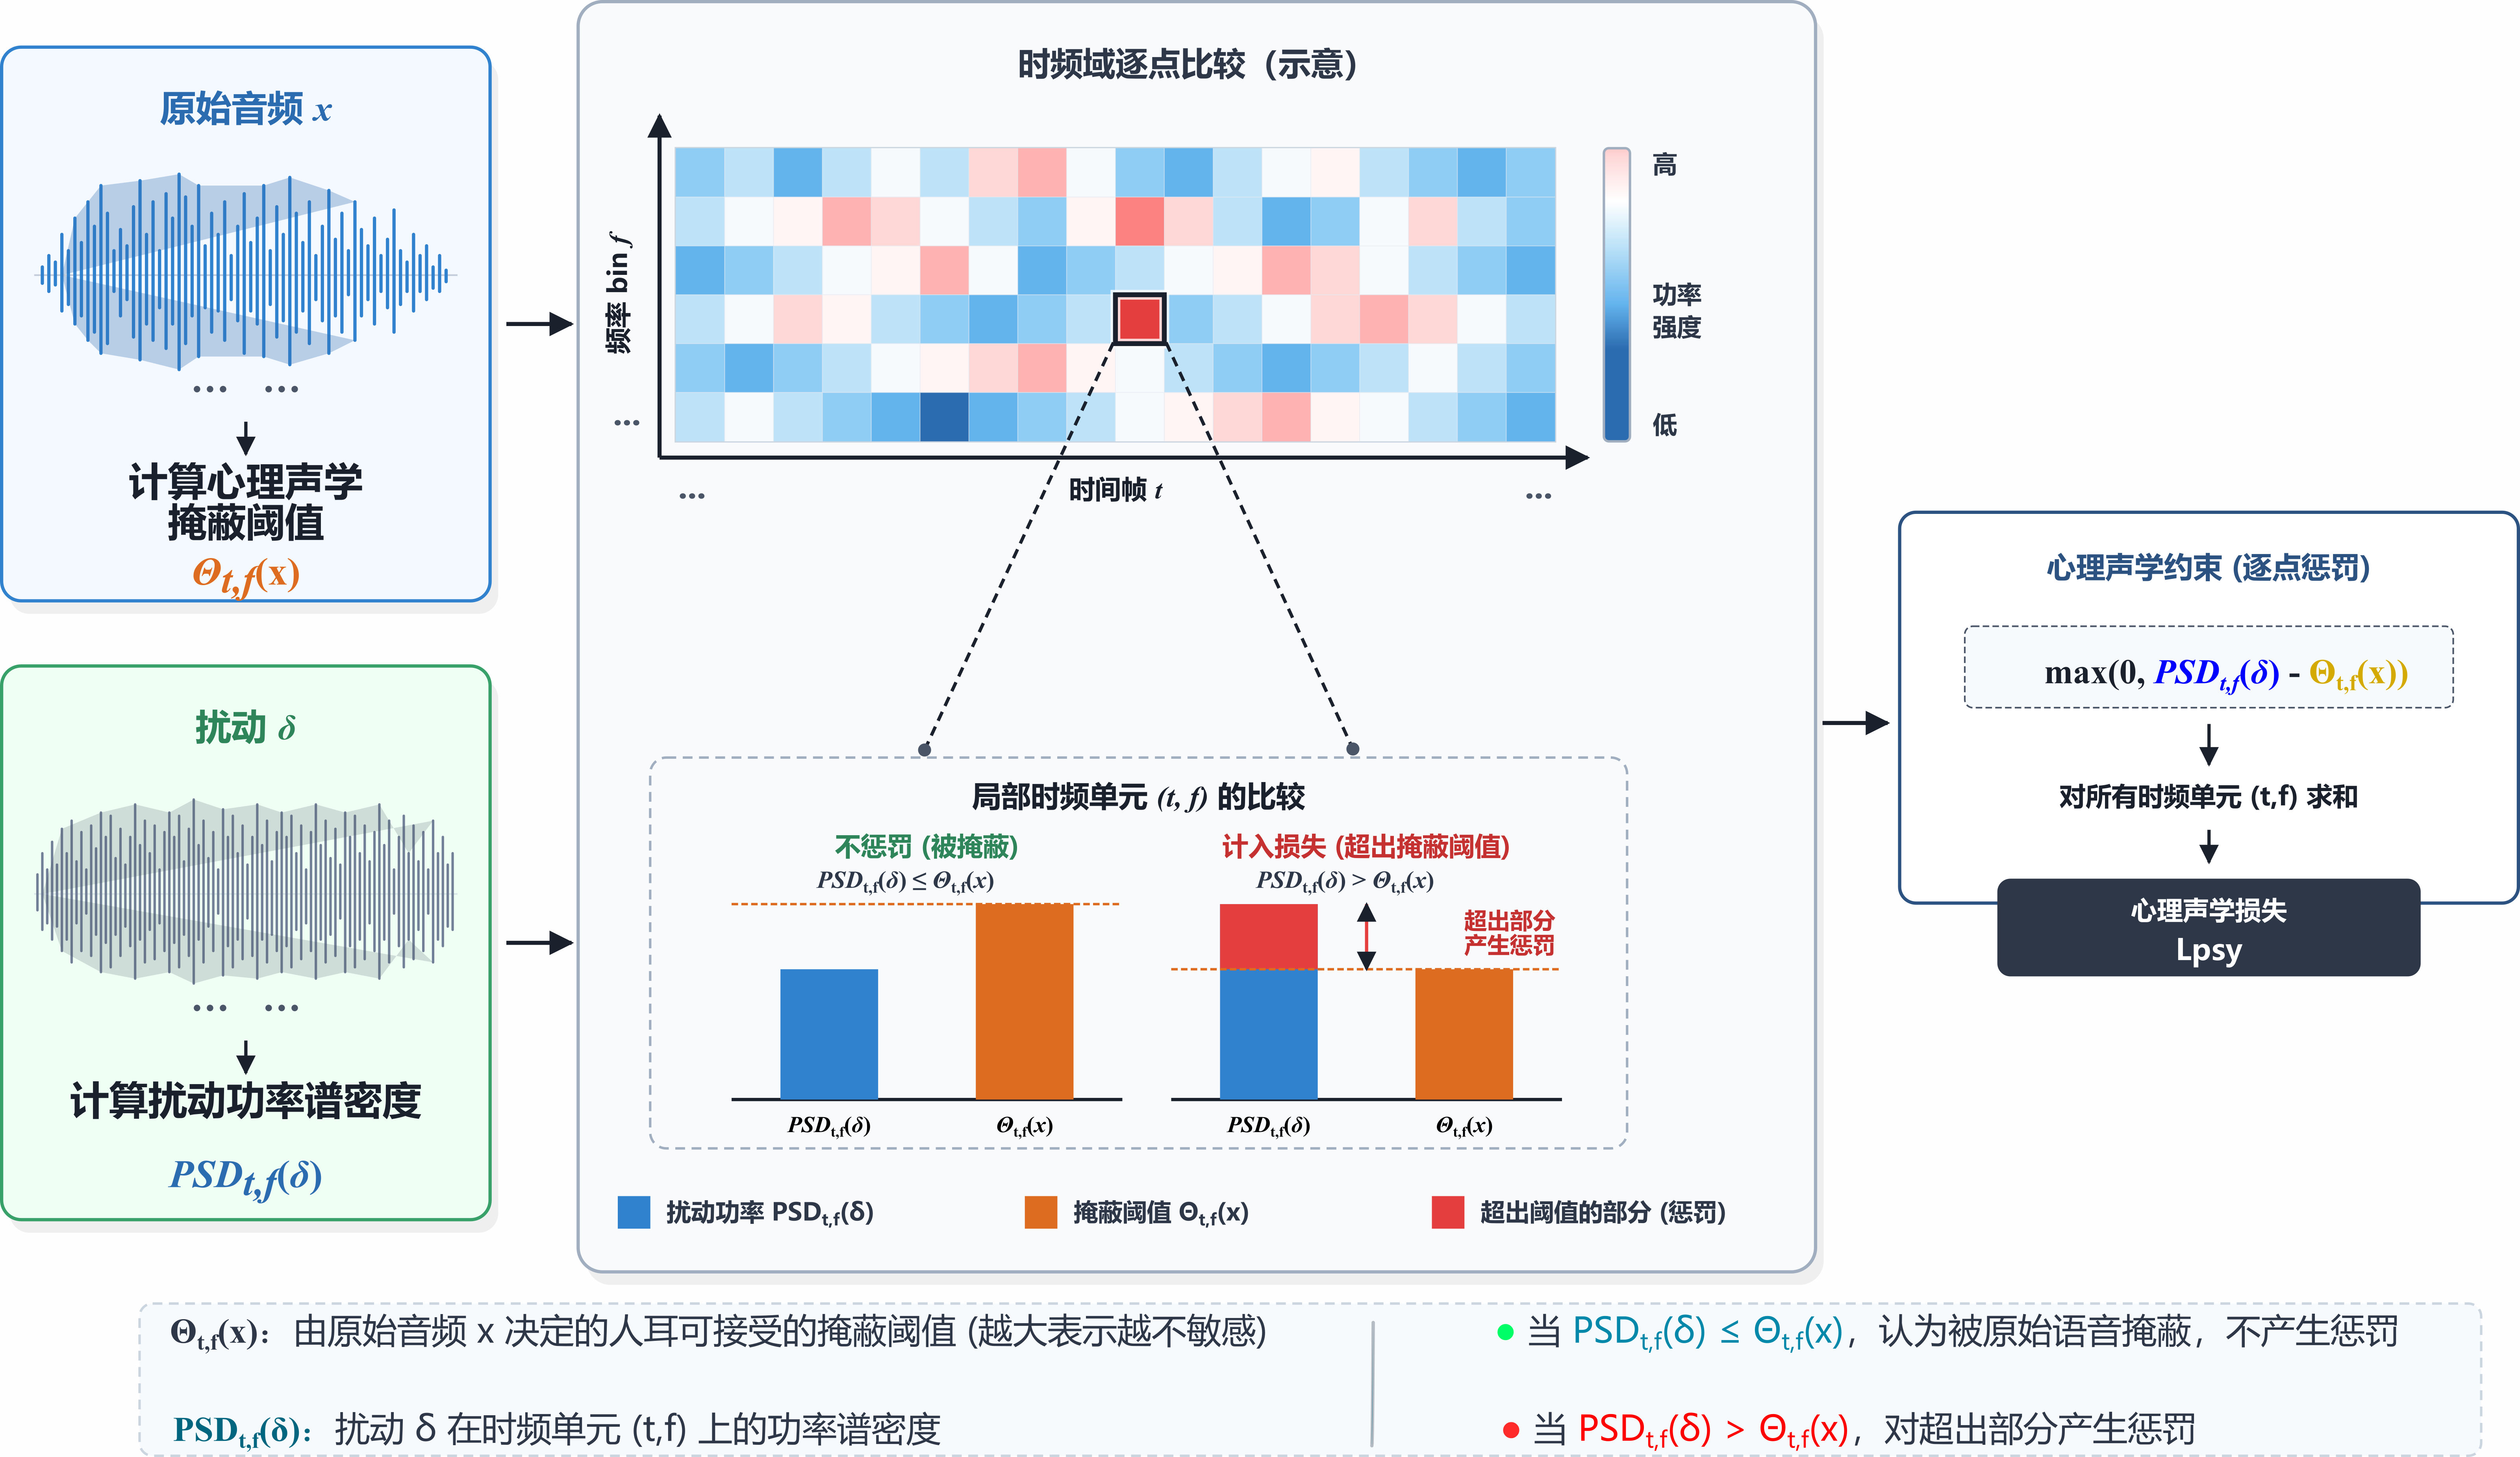
\includegraphics[width=\textwidth,height=0.72\textheight,keepaspectratio]{figures/image21.png}
  \caption{心理声学掩蔽约束计算示意图}
  \label{fig:3-7}
\end{figure}

上述 \(\mathcal{L}_{psy}\)
的含义是，只惩罚``超过听觉掩蔽阈值''的扰动能量。如果某个时频位置上的扰动能量低于
\(M_{x}(t,\ f)\)，则该位置不产生额外听感惩罚；如果扰动能量超过阈值，则超过部分会被加入损失函数。这样可以引导扰动尽量分布在原始语音能量较强、人耳相对不敏感的位置，而不是平均扩散到所有频率区域。

除听感约束外，系统还需要扰动幅度控制。听感约束强调扰动是否容易被人耳感知，而幅度控制强调扰动整体是否过大。二者并不重复：某些扰动即使分布在相对不敏感的频段，如果整体能量过强，也可能造成波形失真、削波或播放异常。因此，系统引入幅度损失项
，用于限制保护音频与原始音频之间的整体差异。感知相关的音频对抗研究也表明，扰动范数与人耳感知质量之间存在密切关系，需要在扰动强度和感知可用性之间进行权衡\textsuperscript{{[}54{]}}。较常用的形式是
幅度约束：

\[\mathcal{L}_{2}\  = |\delta|_{2}^{2}\]

其中，\(|\delta|_{2}^{2}\)
表示保护扰动在时域上的平方能量。该项越大，说明保护扰动整体能量越强；优化过程中增大该项权重，可以使系统生成更小幅度、更保守的保护扰动。

在需要更严格限制单个采样点变化时，系统还可以配合 \(L_{\infty}\)
约束，即要求扰动在任意采样点上的绝对值不超过给定上限：

\[|\delta|_{\infty}\  \leq \ \epsilon\]

其中，\(\epsilon\)
表示允许的最大采样级扰动幅度。该约束通常通过投影操作实现。每轮扰动更新后，系统将
\(\delta\) 裁剪回 \(\lbrack - \epsilon,\epsilon\rbrack\) 范围内：

\[\delta\  \leftarrow \ {Clip}_{\lbrack - \epsilon,\epsilon\rbrack}(x\  + \delta)\]

随后，系统还需要将受保护音频裁剪到合法波形范围内，避免输出音频超过播放器或音频文件格式允许的取值范围：

\[x'\  \leftarrow \ {Clip}_{\lbrack - 1,1\rbrack}(x\  + \delta)\]

其中，\(\lbrack - 1,1\rbrack\)
表示归一化波形常用的合法取值区间。通过扰动裁剪和波形裁剪，系统可以避免保护扰动在迭代优化过程中不断累积，导致音频失真或数值越界。

综合来看，听感约束和扰动控制在系统中分别承担不同职责。
主要约束扰动在时频空间中的可感知性，使扰动尽量避开人耳敏感区域； 和
约束主要控制扰动整体强度和单点幅度，避免波形产生明显失真。该设计与现有语音保护和音频对抗研究中``机器侧效果---人耳侧质量''共同优化的思路一致\textsuperscript{{[}50,53-54{]}}。

\section{系统功能实现}\label{ux7cfbux7edfux529fux80fdux5b9eux73b0}

前文详细阐述了多维特征错位与心理声学约束的理论模型，确立了系统的核心防御策略；同时从工作流程的角度，将
V-Guard
划分为六个核心功能模块。本节的重点在于论述如何将这些处于概念验证阶段的理论模型与抽象功能设计，转化为实际可运行、可部署的工程应用系统。

在真实的业务环境中，防御系统必须直面网络高并发与大算力消耗带来的复杂性。系统构建的核心在于跨越从``单一模型实验验证''到``生产级多维异构联合防御引擎''的工程鸿沟，具体需要解决多架构代理模型的联合集成、极度非凸空间下的多目标寻优平衡，以及有限消费级显卡算力下的显存约束等一系列核心技术问题。

为清晰阐述上述工程细节，这六大功能模块的完整落地将依托于后端底层算法引擎与前端应用交互层的深度解耦来实现。

本节将聚焦于这些模块在后端计算架构与底座算法侧的支撑，其中3.4.1 与 3.4.2
节对应``接入预处理''与``主动保护生成''模块的底层数据流转及寻优解法；3.4.3
节统一阐述``ASR模块''、``身份相似度模块''及``音频质量模块''三大评估模块在后端的自动化度量闭环；3.4.4
与 3.4.5 节则剖析后端如何通过异步推流与接口适配，为``Web
交互与导出模块''提供稳健的高并发底座支撑。通过客观呈现进程隔离、计算图解耦、自适应寻优衰减等具体技术决策过程，展示系统在保障防护效果的同时，如何实现计算资源的高效利用与用户界面的高可用性。

\subsection{后端数据流转控制}\label{ux7aefux5230ux7aefux6570ux636eux6d41ux8f6cux63a7ux5236}

常规学术研究中的对抗样本生成任务通常以单一脚本的形式在静态离线数据集上运行。而在实际业务场景中，防护系统必须提供稳定、持续的在线服务，这意味着系统不仅要处理多源异构的音频格式上传，还需在不阻塞主线程的前提下执行高密度的
GPU 张量运算。为了解决高计算负载带来的 API
阻塞风险，系统采用了前后端深度解耦的分布式架构，结合 React 前端与
FastAPI 后端，实现了计算密集型任务与 I/O
密集型交互的有效隔离。下面这张图详细的展示了系统全链路防克隆数据流转过程：


\begin{figure}[htbp]
  \centering
  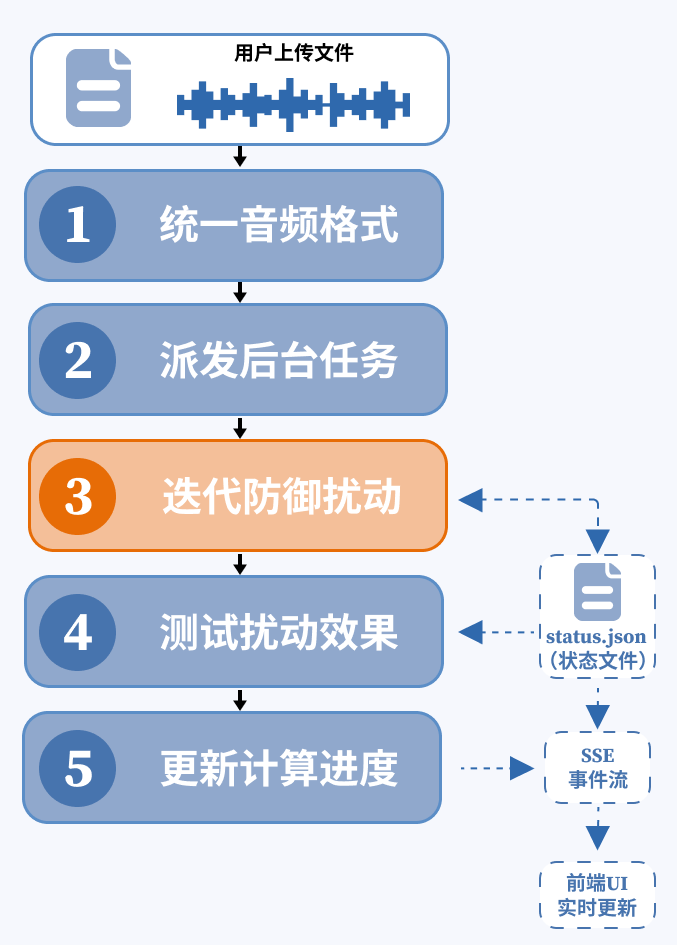
\includegraphics[width=\textwidth,height=0.72\textheight,keepaspectratio]{figures/image22.png}
  \caption{平台端到端音频数据流转过程}
  \label{fig:3-8}
\end{figure}

在该系统架构中，各个层级职责明确，数据流转清晰，共同构成了一个全链路的防克隆保护闭环：

\begin{enumerate}
\def\labelenumi{\arabic{enumi}.}
\item
  音频标准化摄入层

  前端采用流式传输将用户的原始音频数据发送至服务器。鉴于输入音频在编码格式、采样深度及采样率上存在高度不确定性，后端服务在接收数据后，首先介入预处理管线。该管线统一对音频信号进行解码去噪，并将采样率归一化为
  16kHz 的单声道波形序列，进而将其转换为符合 PyTorch
  规范的浮点张量结构。此阶段的严格格式化操作是保障后续多组特征编码器不发生输入不对齐异常的先决条件。
\end{enumerate}

2. 异步调度中心与任务解耦\\
由于多维对抗优化的单次迭代可能耗时数分钟，传统的 HTTP
阻塞式请求/响应模型容易导致网关超时并耗尽连接池。为此，系统服务端引入了异步任务状态机机制。当格式化后的音频到达调度中心时，主服务（FastAPI）会通过多进程模块（multiprocessing）为其拉起独立的守护计算进程，并即时向前端返回任务追踪标识（Task
ID）。主服务不再被计算阻塞，从而保障了 Web API 层的高并发承载力。

3. 对抗寻优计算层\\
独立进程接管计算任务后，初始化核心对抗寻优引擎。引擎在受限的显存空间内，并行调度多路基于
PyTorch 和 ONNX
生态的深度编码器（涵盖语义提取与音色表征）。通过在迭代过程中实时计算梯度并更新输入音频张量，引擎以多目标损失最小化为导向，结合心理声学频域掩蔽模型的实时校验，动态生成扰动噪声，逐步完成原始音频的防御性加噪。

4. 自动化威胁评估与度量闭环\\
为确保防护音频在真实的下游管线中具备实际拦截效果，系统在计算引擎后置了自动化测试沙箱。生成的防御音频会被即时送入内置的声纹识别网络（如
ECAPA-TDNN）与语音识别模块（如
Whisper），通过对克隆前后的语义错误率及声纹相似度衰减进行量化评估，构建起攻防闭环验证体系。

5. 状态同步与持久化分发\\
由于底层算法产生了海量的时序张量与中间评估指标，若直接进行跨进程传递极易导致内存泄漏。系统采用基于文件系统的持久化策略，将计算进程产生的降采样状态数据（status.json）序列化写入磁盘。服务端的调度层利用
Server-Sent Events (SSE)
轮询读取该状态机文件，将进度增量和收敛曲线以极低的开销推送到前端。前端基于
Zustand
状态管理库捕获事件流，在缺失关键指标时执行鲁棒的降级渲染，从而实现了数百步优化过程的大屏实时平滑可视化。

\subsection{算法的计算优化}\label{ux6838ux5fc3ux7b97ux6cd5ux7684ux8d44ux6e90ux7ea6ux675fux4e0eux5e95ux5c42ux4f18ux5316}

本节重点论述系统如何将``多维异构联合防御''理论转化为在有限算力下稳定、高效运行的工程化防御引擎。面对多模型集成所伴随的硬件资源约束与高维空间优化困境，系统在底层防护算法中实施了三项关键的工程决策。

1. 跨架构多大模型的显存危机与集成破局

第二章的理论模型指出，消除防御盲区需要集成涵盖语义理解与音色特征的十余路模型（如
Whisper, HuBERT, WavLM
等）。然而，在常规消费级计算节点上，同时进行多模型的加载与反向传播会引发严重的显存溢出（OOM）。

为解决这一资源瓶颈，系统从计算图结构入手，实施了以下工程解法：

（1）计算图绝缘与梯度冻结：为免除庞大的优化器状态开销，系统在初始化阶段对所有特征提取网络执行参数冻结操作（设定
requires\_grad=False）。在此架构下，优化靶点完全由模型权重转移至输入音频的波形张量（设定
requires\_grad=True）。该策略在保留对抗微扰求导路径的同时，大幅缩减了反向传播期间的显存占用，使得多模型并行优化成为可能。

（2）跨框架动态计算图桥接：为引入部分前沿推理专用模型（如以 ONNX
格式发布的 CAM++），系统集成 onnx2torch 组件。该组件能够在内存中动态解析
ONNX
静态计算图，并将其重构为兼容自动求导协议的动态计算图，从而实现了跨框架组件间梯度回传路径的统一。

（3）松耦合注册表机制：系统通过动态注册与按需加载设计代理模型网，使防御系统能够基于部署环境的可用显存进行伸缩调度，提升了算法层在不同算力设施上的适应性。

\begin{enumerate}
\def\labelenumi{\arabic{enumi}.}
\setcounter{enumi}{1}
\item
  极度非凸空间下的多目标对抗寻优
\end{enumerate}

针对多维异构特征防御，其目标函数涉及语义错位、音色推远及L2范数约束等多个维度的联合优化。该优化空间呈现典型的高维非凸特性，极易陷入使得单一模型误判的局部极小值。为了保证保护效果的平衡，系统在对抗微扰的求解环节中进行了针对性的优化：

（1）基于平台检测的自适应衰减策略（Plateau-based
Decay）：在基础投影梯度下降（PGD）算法上，系统引入了学习率的动态自适应调度。引擎实时监控目标损失函数的收敛趋势，当连续多步观测到损失未能实质性下降时，触发学习率减半机制。该策略有效削弱了优化迭代后期的梯度震荡现象，加速了算法向全局较优解收敛。

（2）高敏感度网络降权与梯度深潜：针对轻量且对微小扰动敏感的网络结构（如
CAM++），其梯度极易主导整体更新方向，导致算法陷于局部最优。系统在计算音色推远的聚合目标函数时，通过引入惩罚机制人为降低此类高敏感网络的余弦损失权重（乘以
0.5
衰减系数）。这种不对称的权重分配强迫优化算法跨越高敏感浅层区域，引导对抗微扰能量向网络更深层（如
WavLM）渗透，从而确保全局对抗泛化能力的提升。

\begin{enumerate}
\def\labelenumi{\arabic{enumi}.}
\setcounter{enumi}{2}
\item
  心理声学约束的动态嵌入
\end{enumerate}

防御体系的隐蔽性要求对抗微扰能量必须严格限制在人耳听觉感知阈值以下。系统需要确保在迭代寻优过程中，每一次计算产生的对抗噪声都不会超越声学限制。

系统通过频域掩蔽校验的内联投影（Projection）将听觉约束深度嵌入至优化器的内部循环。在
PGD
算法的每步前向更新操作后，系统不仅执行常规的范数截断，更引入了基于物理意义的频域校验逻辑。引擎实时转换当前波形并提取扰动功率谱密度（PSD），与系统依据原始音频预提取的掩蔽阈值进行比对。一旦局部频段的扰动功率超出听觉掩蔽的红线，系统立刻触发截断惩罚机制。该工程实现通过绝对的物理边界介入，在不终止算法迭代的前提下，确保了防御系统的对抗强度与隐蔽性的有效平衡。

\subsection{防御效果自动化评估}\label{ux653bux9632ux9a8cux8bc1ux6c99ux7bb1ux4e0eux591aux7ef4ux6548ux80fdux5ea6ux91cf}

在对抗攻击的工程实践中，防克隆技术的有效性无法仅依赖对高维特征向量的初步观测或理论推导来评判。为确保系统输出的音频具备真实的抗攻击与防滥用能力，本系统在整体架构末端构建了自动化的威胁验证与度量闭环。该模块作为量化的防御测试靶场，将生成的保护音频直接投递至真实环境的下游克隆与识别管线中，进行全自动的闭环检验。系统的度量验证机制主要分为两条并行的测试链路，分别针对语音语义与说话人身份两个核心维度进行测试。

\begin{enumerate}
\def\labelenumi{\arabic{enumi}.}
\item
  语义崩塌验证链路

  系统内部集成并内嵌了开源的 Whisper
  语音识别模型，将其作为标准的转写探测引擎。在评估阶段，系统自动化并行处理原始音频与保护音频，分别进行语音到文本（ASR）的转换。为了将语义受损程度进行直观的工程呈现，前端渲染层深度引入并定制了文本
  Diff
  对比算法。该算法通过动态计算两个转写序列之间的最长公共子序列（LCS），对文本中的漏字、错字以及语义倒置现象进行高亮标注。在此基础上，系统通过标准化公式量化计算词错率（WER,
  Word Error Rate）与字错率（CER, Character Error
  Rate）。该指标直接反映了防御微扰如何在听觉不可见的频段内，成功使深度学习模型的声学特征提取发生错乱，客观展示了模型理解受保护音频时的语义解析失效程度。
\item
  音色阻断验证链路

  防止非法音色特征的提取是抗克隆防护的核心目标。为闭环验证该能力，系统级联了下游主流的零样本语音合成模型（如
  XTTS-v2 等）作为模拟攻击载体。系统将被保护音频作为参考音频（Reference
  Audio）送入该 TTS
  模型进行语音克隆尝试。随后，系统提取克隆生成的产物音频以及原始说话人音频，将两者统一送入
  ECAPA-TDNN
  声纹识别网络进行深度特征嵌入（Embedding）提取与余弦相似度计算。基于该流程，系统提取并呈现关键的业务度量指标------声纹相似度下降率（SimDropRate）。通过该项指标，系统得以精确评估保护微扰对声音特征提取网络所造成的破坏力，验证防御机制是否能够实质性阻断未授权的音色复刻。
\end{enumerate}

通过这套双链路的自动化度量机制，系统不仅完成了对抗微扰生成的本职工作，更在工程层面将深奥的防御效果转化为客观、可感、可量化的数据指标。这一机制不仅为防御策略的迭代优化提供了可靠的数值依据，也为系统的最终使用者提供了完整透明的``攻-防-评''对抗实效证明。

\subsection{异步调度架构与状态同步}\label{ux5f02ux6b65ux8c03ux5ea6ux67b6ux6784ux4e0eux9ad8ux53efux7528ux72b6ux6001ux5c55ux793a}

由于多维异构联合防御需要在极度非凸的特征空间中寻找最优微扰，其底层运算属于典型的计算密集型任务。单次音频防护往往需要经历数百步的投影梯度下降（PGD）迭代，并伴随实时心理声学掩蔽阈值的功率谱校验，整体耗时通常达数分钟。在真实业务场景中，若采用传统的
HTTP 同步阻塞模式（Blocking
I/O）处理此类请求，不仅会导致前端由于请求超时而发生交互假死，更会严重阻塞服务端的网关线程，引发雪崩效应。此外，算法在长达数分钟的迭代过程中会产生海量的时序收敛数据，若将其全量推送至前端，将带来极大的网络传输压力，并极易引发浏览器渲染进程的内存溢出（OOM）及页面卡顿。

针对上述工程性能挑战，系统在前后端交互架构与底层数据流转机制上采取了严格的深度工程解耦策略：

(1)
进程隔离与异步状态机协同：在服务端调度层，系统摒弃了传统的同步响应架构，利用
Python 的 multiprocessing.Process
模块，将繁重且耗时的张量计算任务从主事件循环中剥离，隔离至独立的后台工作进程中执行。在此基础上，系统构建了一套基于文件系统的持久化异步状态机（以
status.json 为载体）来承担进程间的状态通信。API
层不再负责等待计算结果，而是转变为轻量级的状态机轮询节点，并通过服务器发送事件（SSE,
Server-Sent
Events）单向通道，将任务的执行进度与阶段性指标毫秒级推流至前端。这一解耦设计将高耗时计算与高并发请求彻底分离，不仅确保了
Web 服务的并发高可用性，同时有效避免了计算波动引发的网络断连。

(2)
海量时序数据的流式处理与高可用渲染：对抗优化过程会高频产出数百步的损失指标与特征变化。若将这些底层海量的原始时序张量无脑堆向
Web 端，不仅会引发网络通道拥堵，还会导致浏览器 UI
渲染线程严重卡顿。为此，系统在底层构建了一套智能的数据抽取管线，精准捕获表征模型收敛状态的关键特征节点并向前端推流。在前端展示层，系统设计了高容错的数据适配接口：面对复杂的网络波动或部分因非标准参数未触发计算的指标，前端组件能够进行状态自适应（如精准提示当前指标获取状态），确保组件按需加载而不会引发局部崩溃。这种底层过滤推流与前端自适应渲染的紧密配合，在捍卫数据链路真实性与客观性的同时，成功支撑起了大屏多维图表（收敛折线、雷达图等）的极度顺滑运转。

\subsection{前后端接口与数据适配}\label{ux524dux540eux7aefux63a5ux53e3ux534fux8baeux4e0eux6570ux636eux9002ux914dux8bbeux8ba1}

前文论述的计算引擎与异步任务调度均在后端服务器深层独立运行，同时系统在前端
UI
与底层算法之间设计了一套标准化、松耦合的接口协议与数据适配层。这一设计有效填补了``底座算法''与``顶层应用展示''之间的工程鸿沟。

1. 基于 RESTful 规范的任务调度接口\\
系统采用前后端完全分离的架构，任务生命周期的管理均通过无状态的 RESTful
API
完成。当前端发起音频保护请求时，并未直接阻塞式调用算法引擎，而是向后端的
/api/protect 接口发送包含原始音频文件与序列化配置参数的
multipart/form-data
请求。服务端接收请求后，执行基础参数校验并拉起独立的异步计算守护进程，随后立即向前端返回全局唯一的任务标识符（Task
ID）。这一请求响应隔离设计，确保了算法层（PyTorch生态）的重度算力波动不会影响网关接口层（FastAPI）的高并发响应能力，为前端工作台界面的即时响应奠定了基础。

2. 基于 SSE 的高频状态推流协议\\
在单次耗时达数分钟的多维对抗寻优迭代中，算法引擎会高频产出大量的中间收敛指标（如联合损失下降轨迹、信噪比变化）。若采用传统的前端轮询（Polling）机制，会造成过高的网络连接开销并带来严重的请求延迟。为此，系统服务端设计了
Server-Sent Events (SSE) 单向推流端点
/api/tasks/\{id\}/events。前端建立持久化长连接后，服务端通过轮询底层的高效状态机文件（status.json），将算法的迭代步数、各维度损失值提取并打包为轻量级事件流推向前端。该协议为
3.5
节中前端收敛折线图、雷达图等大屏组件的毫秒级平滑渲染提供了稳健的数据通道支撑。

3. 面向异构结果的数据适配器（Adapter）机制\\
对抗攻击算法、自动语音识别（ASR）评估链路与语音克隆验证链路的底层输出格式高度异构，它们通常表现为
PyTorch 高维张量、Numpy
数组或物理服务器上的本地绝对文件路径。若将这些未经处理的原生结构直接暴露，将导致前端组件与底层算法高度耦合，任何算法侧的输出调整都可能引发前端界面的渲染崩溃。

为实现彻底的工程解耦，系统在后端的控制层注入了专门的数据适配器组件（result\_adapter.py）。该适配层承担了``数据清洗与格式归一化''的核心职责：

资源路径转换：将所有存储在服务器本地的文件绝对路径拦截，并统一映射为符合
REST 规范的静态资源拉取链接（如
/api/files/\{task\_id\}/...），使得前端音频播放器可以直接流式加载。

指标序列化与精度截断：将底层不同维度的度量指标（如 WER
错误率、SimDropRate 声纹下降率）从复杂的张量类型转化为标准 JSON
浮点数，并统一格式化精度。

异常值安全过滤：对未触发的评估模块或计算异常的指标，强行下发标准化的状态标识符，取代具有误导性的空值或零值。

通过数据适配层这最后一道屏障的过滤与重构，前端交互组件无需理解任何深度学习的计算逻辑。前端仅依赖高度可预期的规范化
JSON 数据结构，即可完成安全、可降级的积木式界面渲染。

\section{系统应用实现}\label{ux7cfbux7edfux5e94ux7528ux5b9eux73b0}

在完成系统总体设计、核心保护机制和主要功能模块实现的基础上，本节进一步从用户使用视角介绍
V-Guard
的应用实现方式。与前述偏向算法原理和后端功能组织的内容不同，本节重点说明系统如何将音频接入、保护任务提交、保护结果分析、历史记录管理和结果文件导出等能力组织为完整的
Web
交互流程，使用户无需直接理解底层模型结构、损失函数或任务调度逻辑，也能够完成声音资产的主动防护操作。

在应用层面，V-Guard
的使用流程围绕``提交任务---生成保护---查看评估---管理结果---导出文件''展开。用户首先在音频保护页面上传待处理音频或视频文件，并根据使用需求选择保护模式和相关参数；系统随后将任务提交至后端服务，由后端完成音频标准化、保护扰动生成和基础指标计算；处理完成后，前端结果分析页面以``保护、ASR、克隆''三个页签集中展示结果。其中，保护页签展示原始音频与受保护音频的试听对比、扰动强度、音频质量、心理声学分析和损失趋势；ASR
页签用于在用户触发 ASR
测试后展示语音识别差异、错误率和语义链路指标；克隆页签用于在用户触发语音克隆测试后展示克隆音频对比、说话人相似度变化、嵌入距离变化和克隆防护雷达图。用户还可以在历史记录页面重新查看已完成任务，并下载受保护音频、评估报告或完整证据链文件。

因此，系统应用实现并不只是对算法输出文件的简单展示，而是将主动语音保护能力封装为面向普通用户的可操作流程。通过可视化页面，系统将复杂的语义表示保护、声音身份特征保护和听感质量约束转化为可配置、可观察、可复查和可导出的应用功能，从而增强作品的工程完整性和实际展示价值。

\subsection{音频保护模块}\label{ux97f3ux9891ux4fddux62a4ux6a21ux5757}

音频保护模块是用户使用 V-Guard
系统的核心入口，主要用于完成待保护音频接入、防护策略配置和保护任务提交。该模块对应前文系统功能实现中的音频接入、参数配置和主动保护生成流程，是用户从``上传原始音频''进入``生成受保护音频''的主要操作页面。

防护工作台页面整体划分为音频接入区、防护策略配置区和系统流程说明区三个部分。


\begin{figure}[htbp]
  \centering
  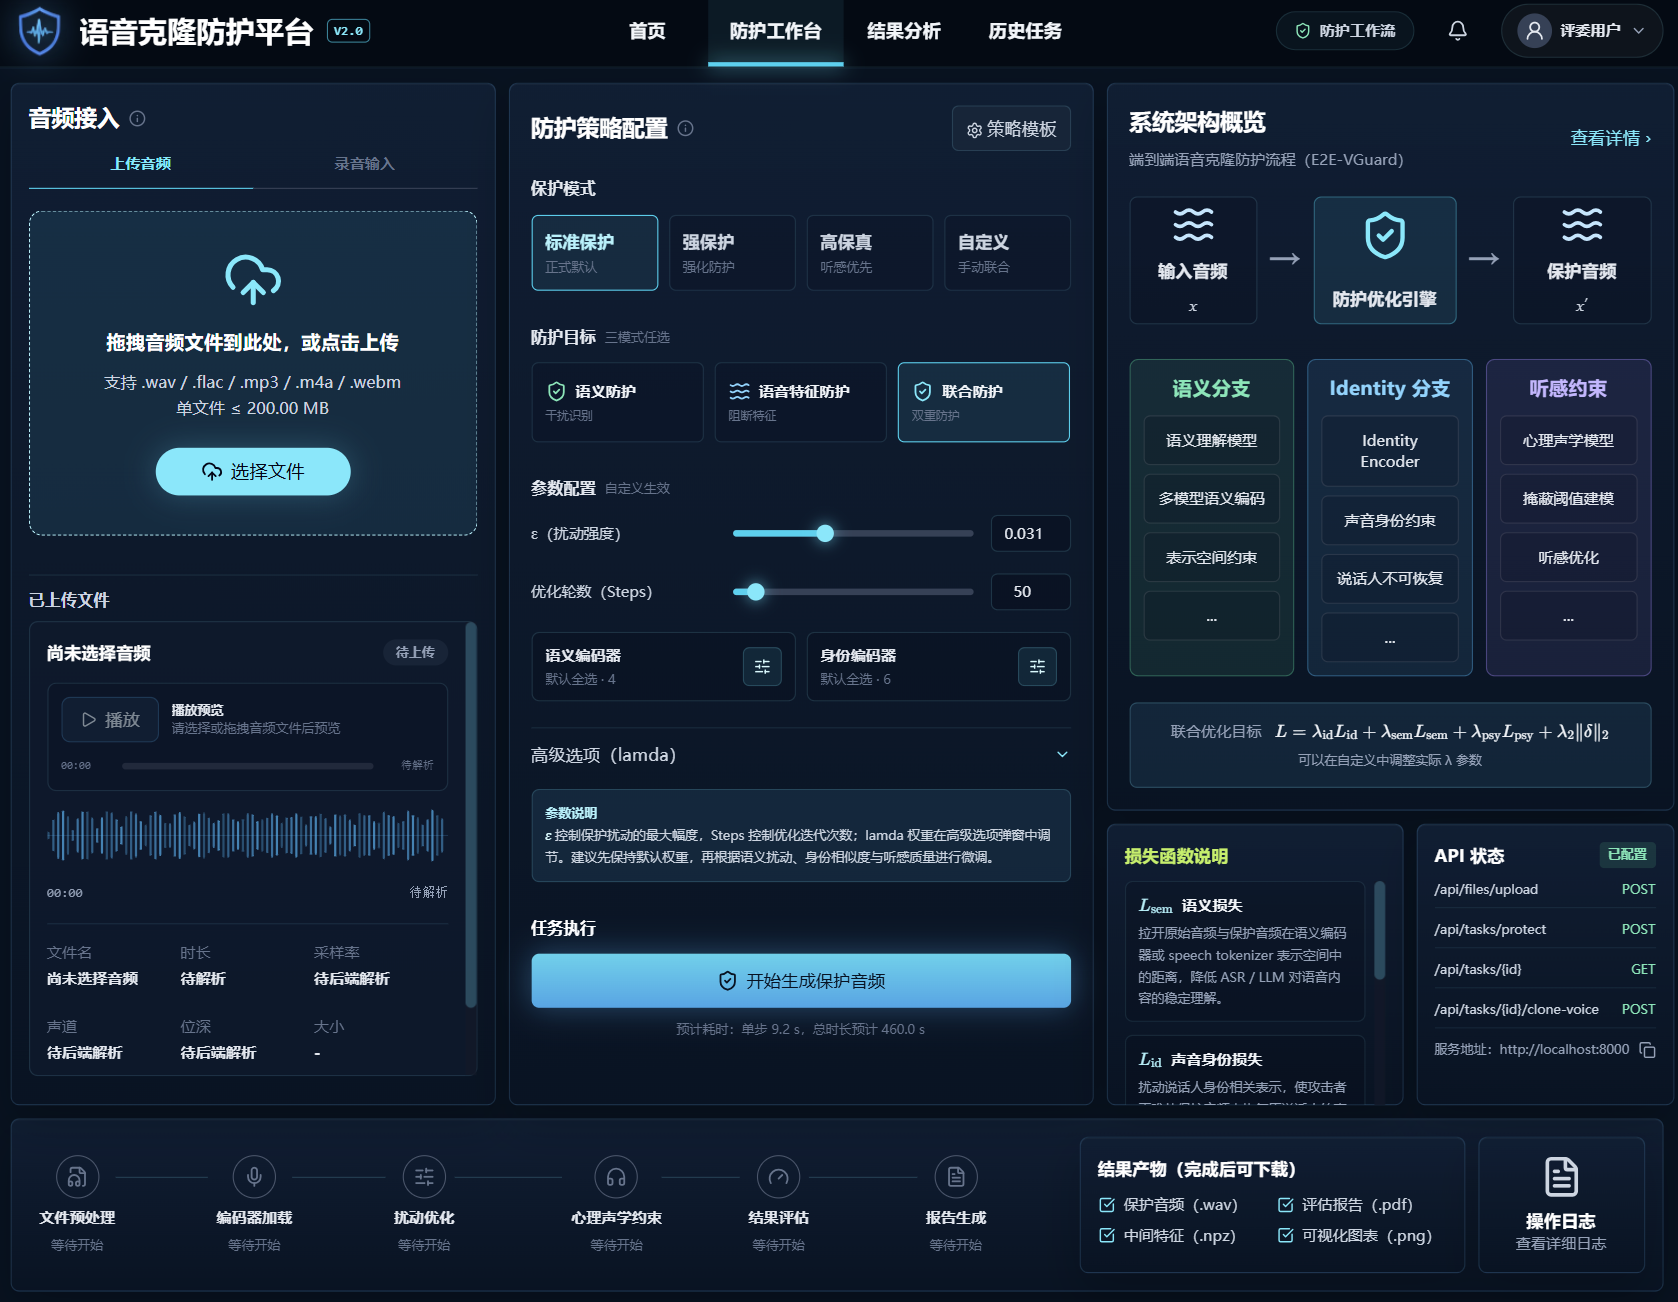
\includegraphics[width=\textwidth,height=0.72\textheight,keepaspectratio]{figures/image23.png}
  \caption{音频保护模块与防护策略配置页面展示图}
  \label{fig:3-9}
\end{figure}

音频接入区用于接收用户上传的原始音频文件，支持用户通过拖拽或点击选择文件的方式导入待保护语音。系统在页面中展示支持的音频格式、文件大小限制和音频预览区域，便于用户在提交保护任务前确认输入文件是否正确。音频上传后，系统会在后端进行格式检查、采样率统一、声道转换和必要的音频标准化处理，将不同来源的语音文件转换为保护算法可处理的标准输入。

防护策略配置区用于控制保护任务的主要参数。用户可以根据使用场景选择不同的保护模式，例如标准保护、强保护、高保真保护或自定义保护。标准保护用于在防护效果和听感质量之间取得默认平衡；强保护更侧重机器侧表示扰乱效果；高保真保护更强调人耳听感质量；自定义保护则允许用户根据实际需求调整部分参数。在保护目标方面，页面提供语义防护、声音身份特征防护和联合防护等选择，其中语义防护主要面向机器对``说了什么''的语义表示链路，声音身份特征防护主要面向机器对``是谁在说、怎么说''的身份、音色、韵律和风格提取链路，联合防护则同时启用语义侧和声音身份侧保护目标。

在参数配置方面，用户可以调整扰动强度、优化轮数以及部分高级参数。扰动强度用于控制保护扰动的最大幅度，优化轮数用于控制保护生成过程的迭代次数。系统在页面中对关键参数给出说明，帮助用户理解参数变化对防护强度、处理耗时和听感质量的影响。对于普通用户，系统提供默认参数和策略模板，降低使用门槛；对于需要实验验证或参数对比的场景，用户也可以通过自定义模式进行更细粒度配置。

用户完成音频接入和策略配置后，可以点击``开始生成保护音频''提交任务。前端会将上传文件和保护参数发送至后端服务，由后端创建保护任务并调用主动保护生成模块。任务执行过程中，系统根据当前配置生成保护扰动，并将扰动叠加到原始音频上，最终得到受保护音频。

保护生成过程对应前文 3.4
节中的主动防护生成模块实现：前端负责收集用户输入和展示任务状态，后端负责执行音频标准化、模型调用、扰动优化和文件保存。

页面右侧的系统流程说明区用于帮助用户理解保护任务的内部逻辑。该区域以简化流程图展示``输入音频---防护优化引擎---保护音频''的基本处理过程，并进一步说明语义表示分支、声音身份特征分支和听感约束在联合防护中的作用。其中，语义表示分支用于降低机器对语音内容、语义表示和语音
token
的稳定建模能力，声音身份特征分支用于削弱机器对说话人身份、音色和风格特征的提取能力，听感约束则用于限制保护扰动对正常收听体验的影响。通过这种可视化说明，系统将底层算法机制转化为用户更容易理解的防护流程。

总体来看，音频保护模块完成了从用户输入到保护任务创建的关键转换。它不仅提供音频上传和参数配置功能，还将语义防护、声音身份特征防护和听感约束等算法能力封装为可选择、可配置、可执行的页面操作。用户无需直接接触底层模型和扰动优化代码，即可通过
Web 页面完成声音资产的发布前主动保护。

\subsection{保护效果展示模块}\label{ux4fddux62a4ux6548ux679cux5c55ux793aux6a21ux5757}

防护结果分析与下游验证模块是系统完成保护音频生成后的核心展示与评估入口。该模块不仅展示保护音频本身，还进一步围绕``保护扰动是否可控、保护音频是否保持可接受听感、ASR
语义识别是否受到影响、语音克隆所依赖的声音身份特征是否被削弱''等问题，对保护结果进行多维度分析。通过该模块，用户能够从单一的音频输出文件进一步获得可试听、可下载、可对比、可解释的实验结果。


\begin{figure}[htbp]
  \centering
  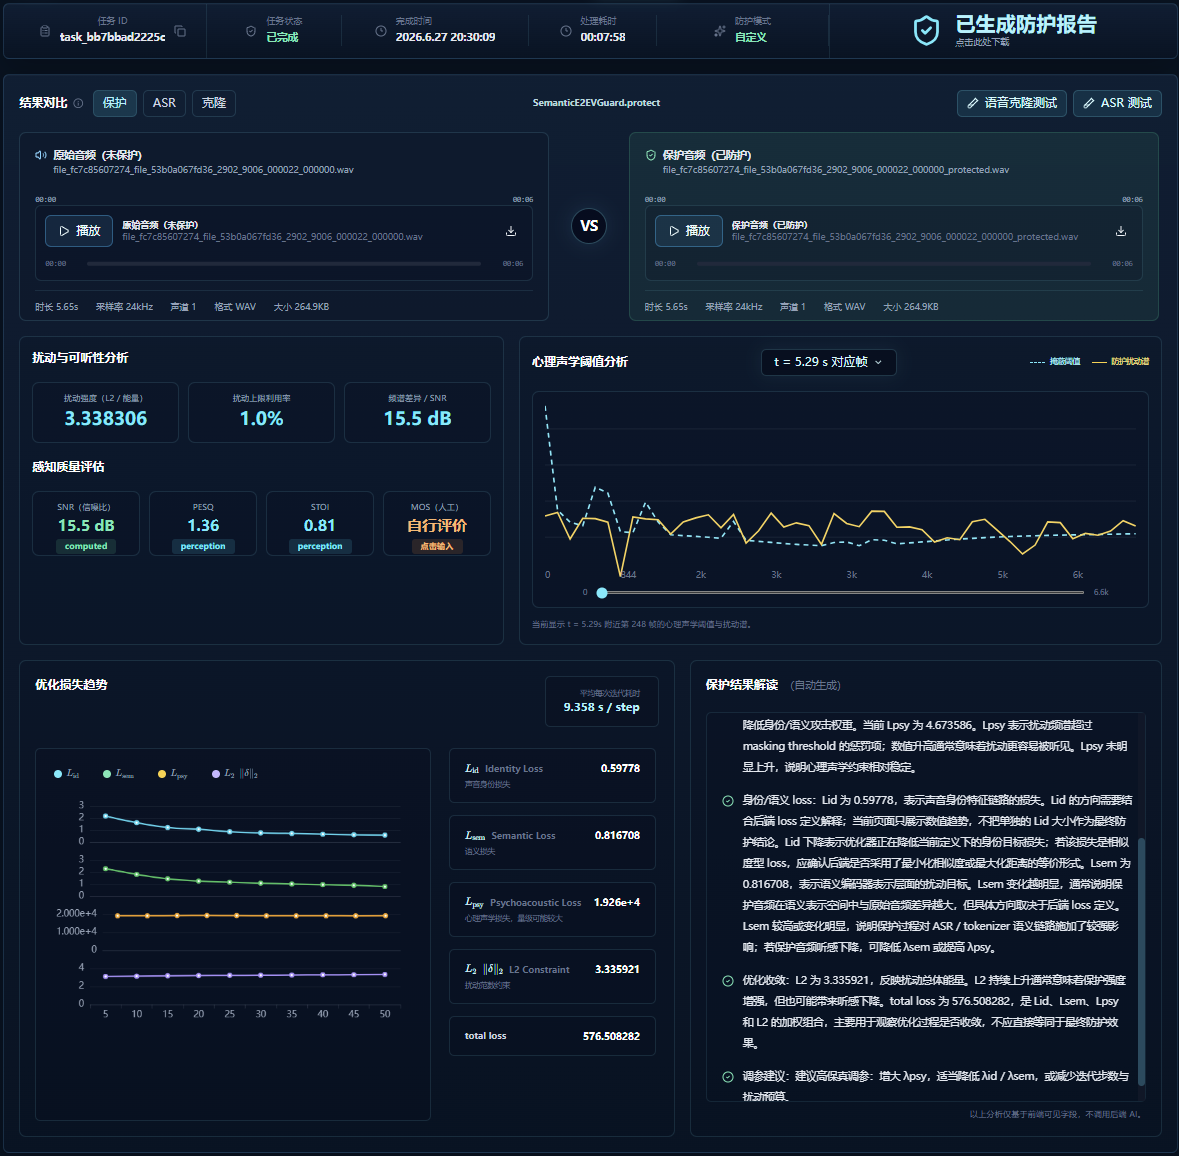
\includegraphics[width=\textwidth,height=0.72\textheight,keepaspectratio]{figures/image24.png}
  \caption{结果分析页面展示图}
  \label{fig:3-10}
\end{figure}

在保护结果分析方面，系统首先对原始音频和保护音频进行并列展示，提供播放、下
载、基础音频属性查看等功能。用户可以直接试听保护前后的音频差异，并查看音频
时长、采样率、声道数、文件格式和文件大小等信息。该设计使保护结果不再只是后
端生成的文件路径，而是转化为可被用户直接验证的应用产物。系统同时展示扰动强
度、扰动上限利用率、信噪比等指标，用于描述保护音频相对于原始音频的扰动规模
和失真程度。

在质量感知评价方面，系统接入了 SNR、PESQ、STOI 和 MOS 等指标，用于从信号
质量、语音可懂度和主观听感估计等角度衡量保护音频的可接受程度。其中，SNR
反 映原始语音信号与扰动噪声之间的能量关系；PESQ 和 STOI
用于评估保护音频在感 知质量和语音可懂度方面的变化；MOS
作为听感等级参考，用于辅助用户判断保护
音频是否仍具备可使用性。通过这些指标，系统能够在``防护强度''和``听感质量''之间
提供更直观的权衡依据。

在心理声学约束分析方面，系统展示掩蔽阈值与防护扰动谱之间的频域关系。该部分
用于反映扰动是否尽可能分布在人耳较不敏感或可被原始语音掩蔽的频段中。相比仅
使用扰动幅度作为约束，心理声学分析能够更贴近人耳感知特性，体现系统在生成保
护扰动时并非单纯追求模型误导效果，而是同时考虑音频自然性和可听性。
在优化过程解释方面，系统记录并展示多目标联合优化过程中的损失变化趋势，包括
身份损失、语义损失、心理声学损失、L2
约束项以及总损失。身份损失用于反映保
护音频在声纹特征空间中对原始说话人身份表征的偏移程度；语义损失用于衡量保护
音频对语义编码器和语音识别相关表示的干扰效果；心理声学损失用于约束扰动的可
感知程度；L2
约束用于限制扰动整体幅度。通过损失趋势展示，用户能够观察系统
在多轮迭代中如何对不同优化目标进行联合调整，从而理解保护音频并非由固定噪声
模板生成，而是由多分支目标共同驱动得到。


\begin{figure}[htbp]
  \centering
  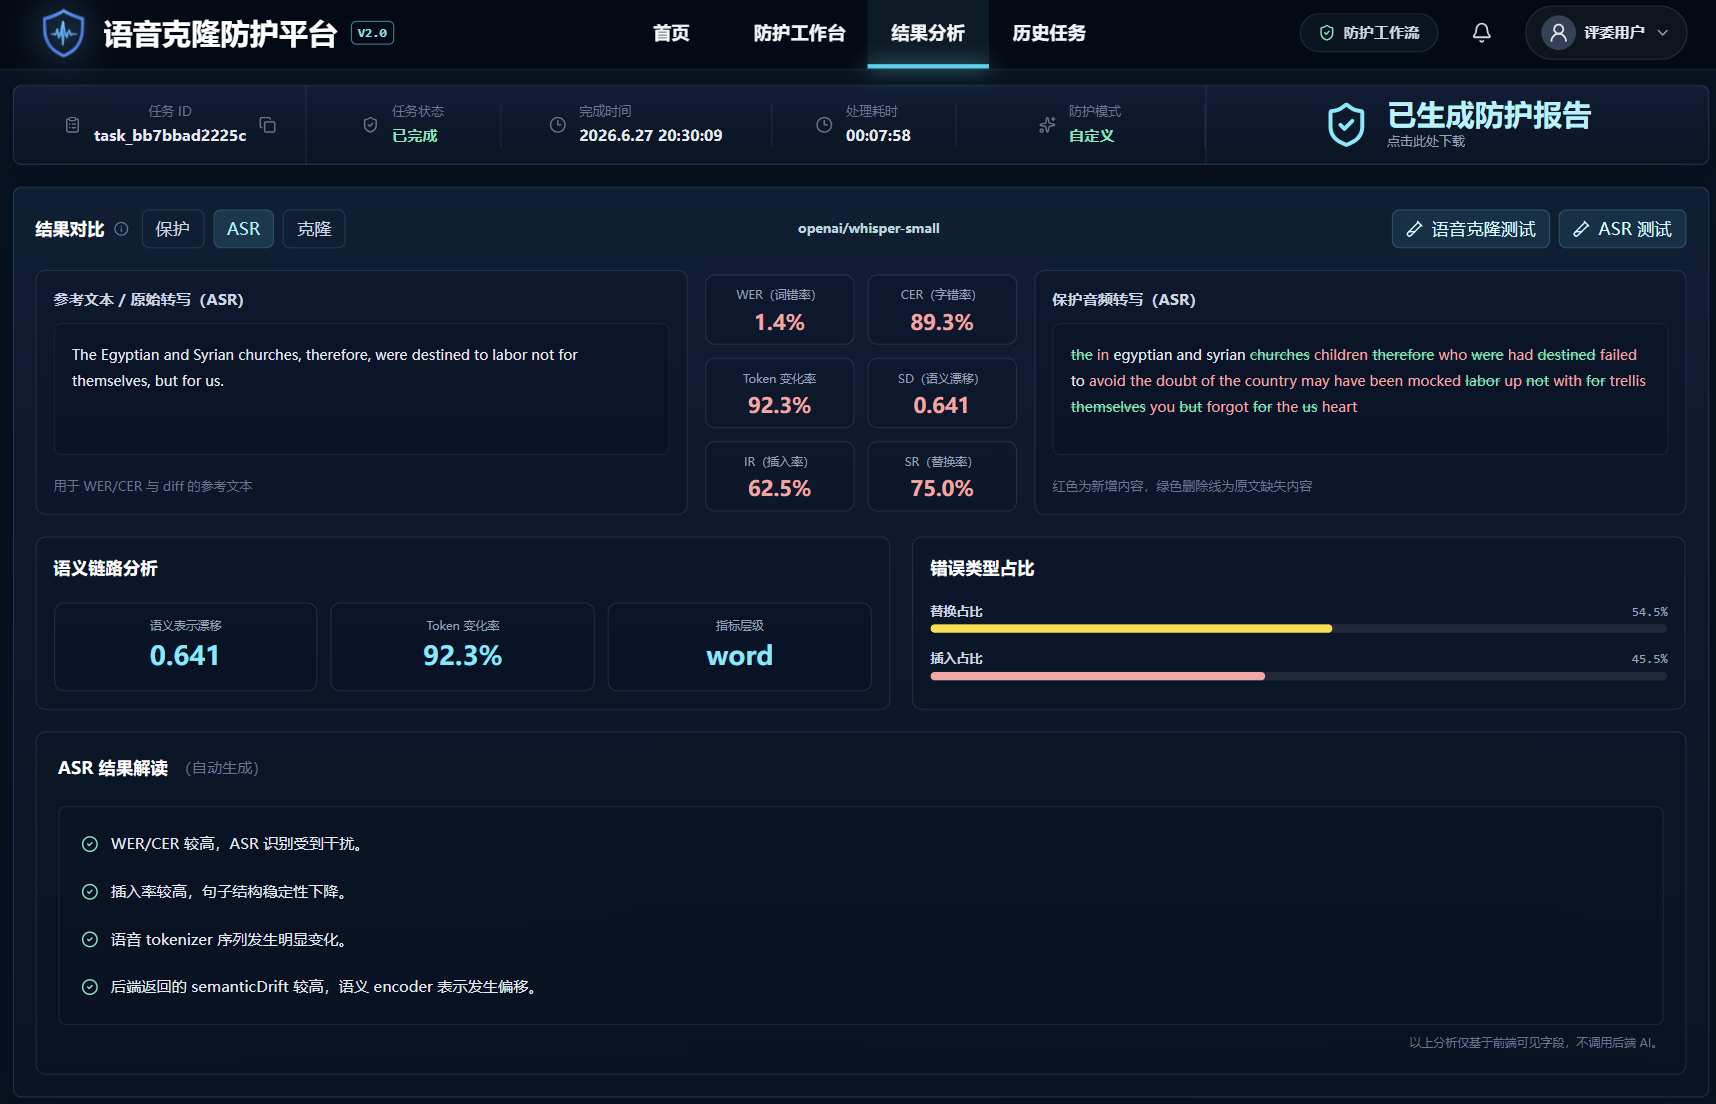
\includegraphics[width=\textwidth,height=0.72\textheight,keepaspectratio]{figures/image25.png}
  \caption{结果分析-ASR分析展示图}
  \label{fig:3-11}
\end{figure}

除保护音频本身的分析外，系统进一步提供 ASR
下游验证功能。用户可以对生成后的保护音频执行语音识别测试，系统会展示原始参考文本、保护音频转写结果以及二者之间的差异。页面通过
WER、CER、Token
变化率、语义漂移、插入率、替换率和删除率等指标衡量保护音频对语音识别模型的影响。文本差异区域使用颜色标注新增内容和原文缺失内容，使用户能够直观看到保护音频在识别结果中引入了哪些错误。该功能对应系统的语义表示保护目标，即通过主动扰动降低攻击者或下游模型对语音内容的可靠识别能力。ASR
验证流程可概括为：

\begin{center}
\fbox{\parbox{0.9\textwidth}{\centering 原始音频/受保护音频 $\rightarrow$ ASR 音频 $\rightarrow$ 转写文本 $\rightarrow$ 文本差异与语义链路指标}}
\end{center}


\begin{figure}[htbp]
  \centering
  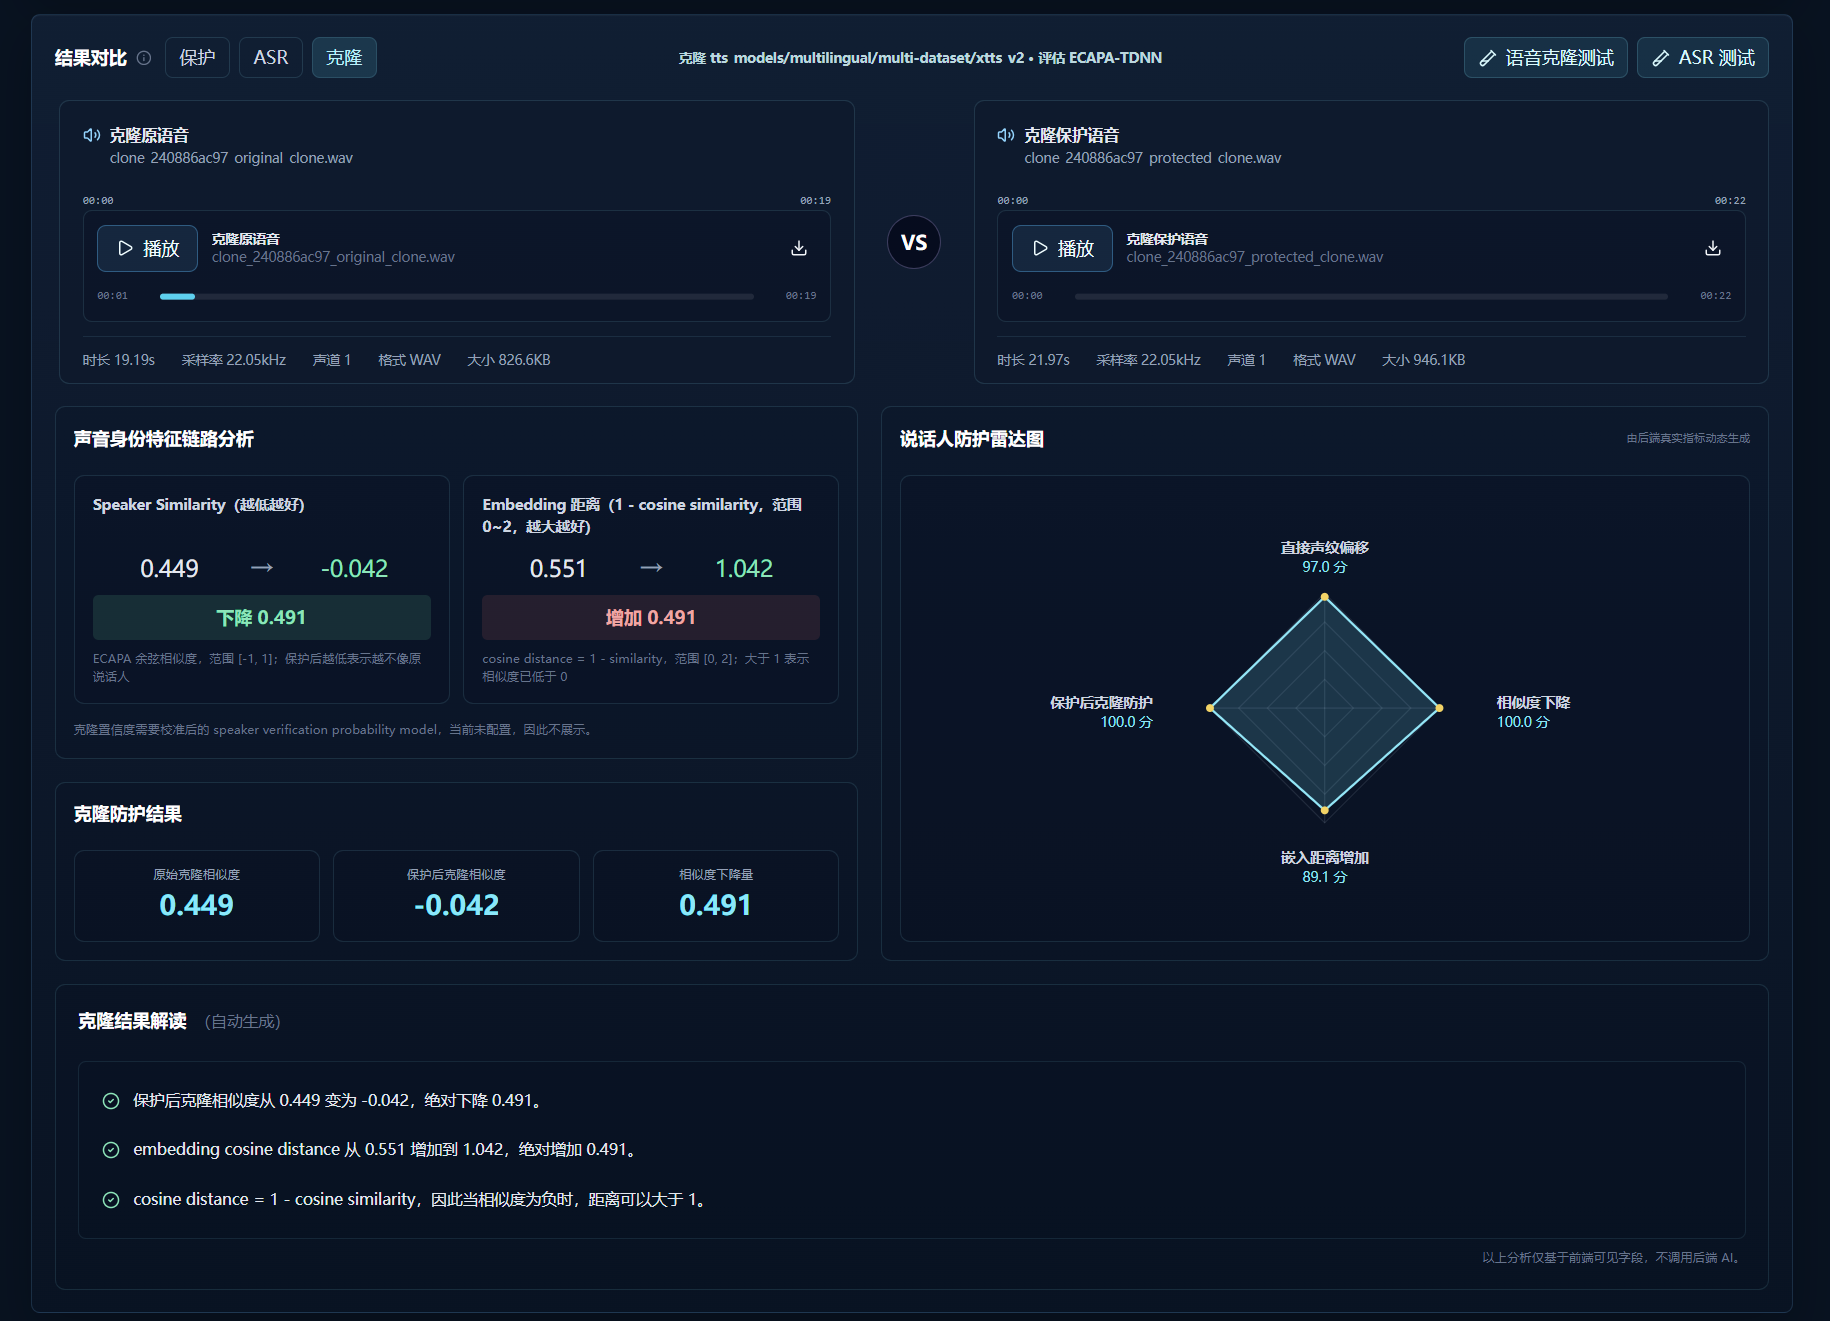
\includegraphics[width=\textwidth,height=0.72\textheight,keepaspectratio]{figures/image26.png}
  \caption{结果分析-克隆分析展示图}
  \label{fig:3-12}
\end{figure}

系统还提供语音克隆防护验证功能，用于评估保护音频对语音克隆链路的影响。用户可以基于原始音频和保护音频分别生成克隆语音，并对两类克隆结果进行对比。系统通过
Speaker Similarity、Embedding
距离、相似度绝对下降量等指标衡量保护前后声音身份特征的变化。如果保护音频导致克隆结果与原始说话人相似度下降、Embedding
距离增大，则说明保护扰动有效破坏了语音克隆模型所依赖的声音身份表征。页面中的雷达图进一步从直接声纹偏移、相似度下降、嵌入距离增加和保护后克隆防护等维度综合展示防护效果。

克隆验证流程可概括为：

\begin{center}
\fbox{\parbox{0.9\textwidth}{\centering 原始音频/受保护音频 $\rightarrow$ 语音克隆模型 $\rightarrow$ 克隆音频 $\rightarrow$ 说话人评估模型 $\rightarrow$ 克隆防护指标}}
\end{center}

为了降低用户理解复杂指标的门槛，系统在各分析页面中提供自动生成的结果解读。该区域会根据当前任务的指标结果，对保护音频是否成功生成、ASR
是否受到干扰、语音克隆相似度是否下降、感知质量是否存在损失等内容进行文字化说明。用户无需直接阅读后端日志或算法调试信息，即可从前端页面理解本次保护任务的主要效果和潜在不足。

综上，防护结果分析与下游验证模块实现了从保护音频生成到效果验证的闭环。系统不仅能够生成受保护音频，还能够进一步从可听性、语义识别偏移和语音克隆防护三个层面验证保护效果，为主动式语音防克隆技术的应用展示和实验对比提供了完整支撑。

\subsection{历史记录查看和结果导出模块}\label{ux5386ux53f2ux8bb0ux5f55ux67e5ux770bux548cux7ed3ux679cux5bfcux51faux6a21ux5757}

历史任务查看与结果导出模块用于对系统已执行任务进行集中管理，并为用户提供结果复查、音频下载和证据材料导出能力。由于主动式语音保护任务通常涉及多轮参数调节、多次模型测试和多组结果对比，单次任务完成后仍需要具备可追溯、可复查和可导出的能力。因此，系统在完成保护音频生成及下游验证后，会自动将任务记录写入历史任务页面，形成完整的任务管理闭环。

历史任务页面按照任务类型对记录进行分类展示，包括保护历史记录、ASR
历史记录和语音克隆历史记录。保护历史记录主要保存音频保护生成任务，ASR
历史记录用于保存语音识别测试任务，语音克隆历史记录用于保存克隆防护验证任务。不同类型任务通过标签页进行区分，使用户能够根据实验阶段快速定位相应结果，避免保护生成、识别评估和克隆评估记录混杂在同一列表中。


\begin{figure}[htbp]
  \centering
  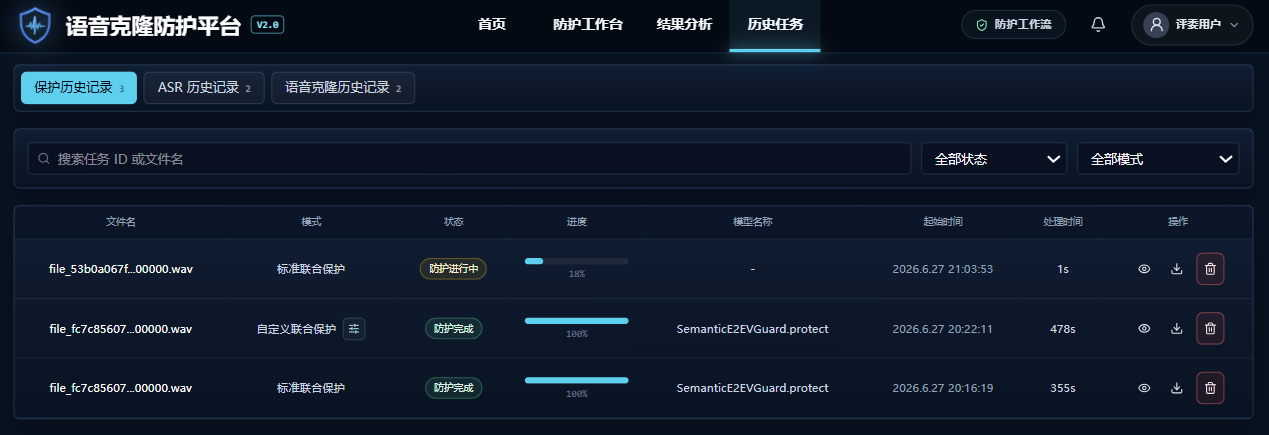
\includegraphics[width=\textwidth,height=0.72\textheight,keepaspectratio]{figures/image27.png}
  \caption{历史任务页面展示图}
  \label{fig:3-13}
\end{figure}

在任务列表中，系统展示文件名、防护模式、任务状态、执行进度、模型名称、起始时间和处理时间等关键信息。任务状态用于标识任务是否正在执行、已经完成或执行失败；进度条用于展示当前任务执行比例；处理时间用于反映算法生成或评估过程的时间开销。对于仍在运行的任务，用户可以在历史页面持续观察其状态变化；对于已经完成的任务，用户可以进一步进入结果页面查看详细分析。

历史任务页面还提供搜索与筛选功能。用户可以根据任务
ID、文件名、任务状态或防护模式对历史记录进行检索，从而快速定位特定实验结果。该功能尤其适用于多次调整优化步数、扰动强度、语义权重或音色权重后的对比实验场景。通过历史记录，用户可以保留不同参数配置下的保护结果，并根据执行时间和任务状态进行复查。

在每条任务记录的操作区，系统提供查看、下载和删除等功能。查看按钮用于跳转到对应任务的结果分析页面，用户可以继续查看保护音频对比、扰动与可听性分析、ASR
识别干扰结果以及语音克隆防护结果。下载按钮用于直接获取该任务生成的保护音频，方便用户将受保护音频保存到本地或用于后续测试。删除按钮用于清理无效、失败或过期任务，避免历史列表长期堆积无关记录。


\begin{figure}[htbp]
  \centering
  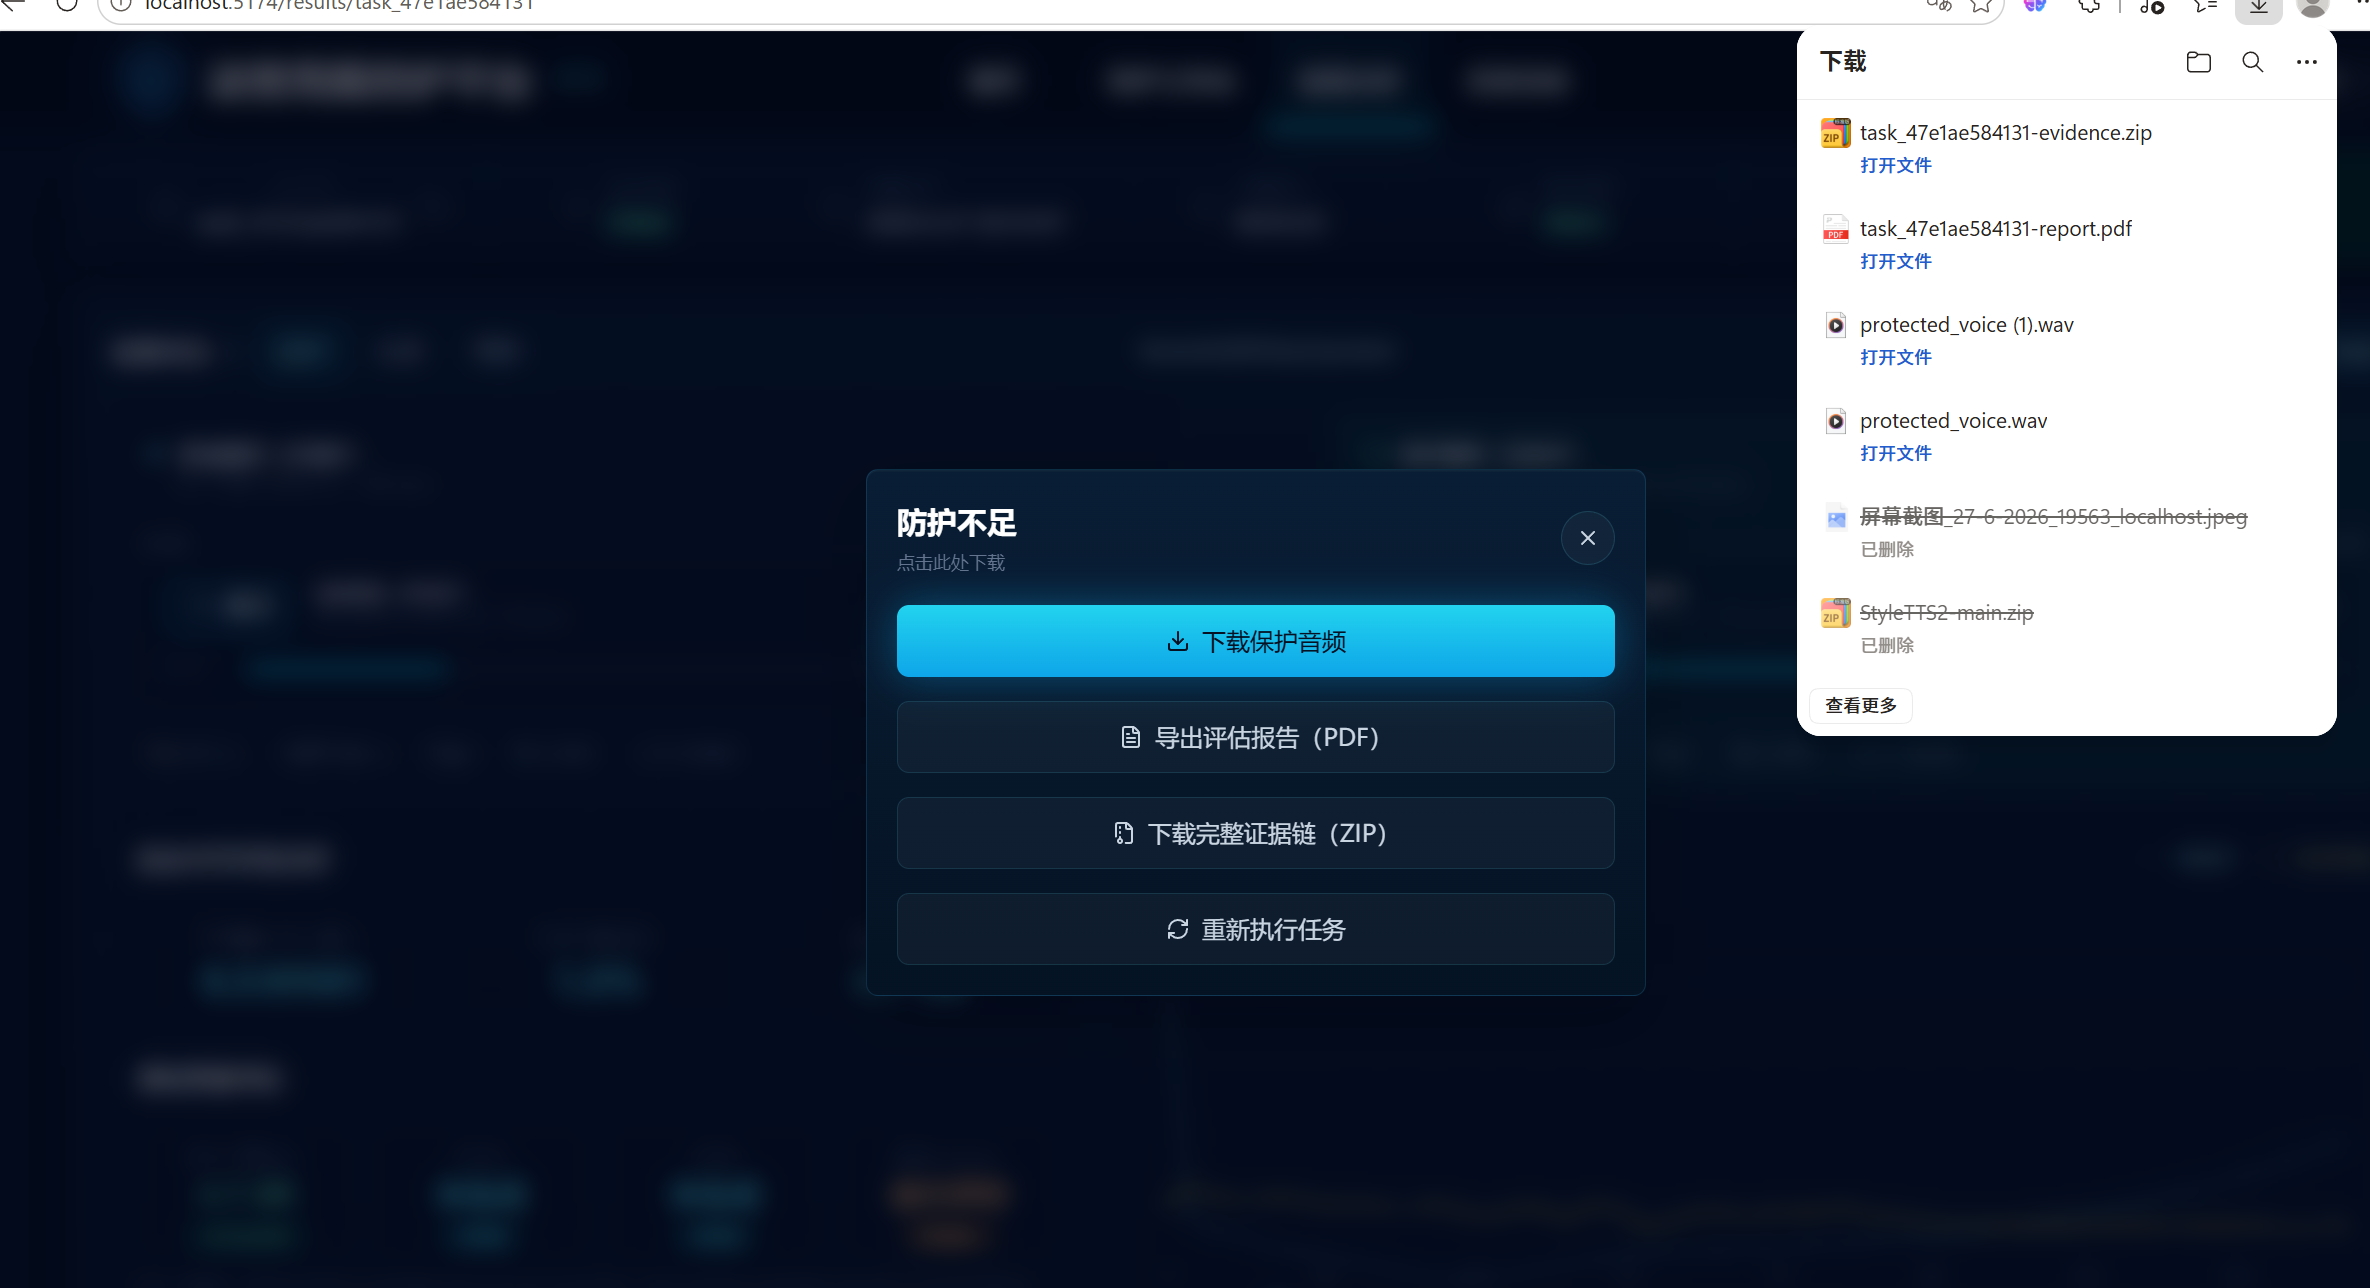
\includegraphics[width=\textwidth,height=0.72\textheight,keepaspectratio]{figures/image28.png}
  \caption{下载结果展示图}
  \label{fig:3-14}
\end{figure}

除历史任务列表中的快捷下载外，系统还在结果分析页面提供完整的结果导出入口。当保护任务完成后，页面右上角会显示防护报告生成状态，用户点击后可以选择下载保护音频、导出评估报告或下载完整证据链压缩包。其中，保护音频用于直接获取系统生成的受保护语音；评估报告以
PDF
形式保存当前任务的关键信息、指标结果和分析结论；完整证据链压缩包则用于打包任务相关文件，便于后续归档、复现实验或提交材料。

结果导出功能使系统不仅能够完成在线展示，还能够生成可离线保存的实验产物。对于竞赛作品和实验报告而言，该功能能够将系统运行结果转化为可提交、可复核的文件材料；对于实际应用场景而言，用户也可以通过导出的保护音频和报告文件，完成后续验证、转发或存档。由此，系统形成了从音频上传、防护生成、结果分析、历史追踪到证据导出的完整应用流程。

整体来看，历史任务查看与结果导出模块提升了系统的工程完整性和可用性。它不仅记录了每次保护与评估任务的执行状态，还提供了任务复查、保护音频下载、PDF
报告导出和证据链打包等功能，使主动式语音防护结果能够被长期保存、重复查看和进一步验证。

\FloatBarrier
